\documentclass[PhD,binding=0cm,noexaminfo,oneside]{sapthesis}
\captionsetup{format=plain,indention=0cm,singlelinecheck=false,justification=raggedright,width=.95\textwidth}
\usepackage{microtype} % http://www.khirevich.com/latex/microtype/
\usepackage[utf8]{inputenx}
\usepackage{hyperref}
\usepackage[numbers,square]{natbib}
\usepackage{algorithm2e}
\usepackage{wrapfig}

\hypersetup{
  colorlinks = true, % colours links instead of ugly boxes
  urlcolor = blue, %  colour for external hyperlinks
  linkcolor = black, % colour of internal links
  citecolor = black, % colour of citations
  pdftitle = {New Techniques for Adaptive Program Optimization},
  pdfauthor= {Daniele Cono D'Elia}
}	

\setcounter{tocdepth}{4}
\setcounter{secnumdepth}{4}

\title{New Techniques for Adaptive Optimization}
\author{Daniele Cono D'Elia}
\IDnumber{1208297}
\course[Computer Engineering]{Ingegneria Informatica}
\courseorganizer{School of Information Engineering, Computer Science and Statistics}
\cycle{XXVIII}
\submitdate{June 2016}
\copyyear{2016}
\advisor{Prof. Camil Demetrescu}
\coadvisor{Prof. Steven Blackburn}
\coadvisor{Dr. David Grove}
\authoremail{danielecono.delia@gmail.com}

\newcommand{\noauthorea}{}
\usepackage{color}
\usepackage{latexsym}
\usepackage{listings}
\usepackage{enumitem}

\let\oldnl\nl% Store \nl in \oldnl
\newcommand{\nonl}{\renewcommand{\nl}{\let\nl\oldnl}}% Remove line number for one line

%\usepackage{algorithm2e}
%\usepackage{tabularx}

% uncomment to enable clever references
\ifdefined\noauthorea
\usepackage{cleveref} 
\AtBeginDocument{\renewcommand{\ref}[1]{\Cref{#1}}}
\AtBeginDocument{\renewcommand{\eqref}[1]{\Cref{#1}}}
\fi

% commands
\ifdefined\noauthorea
\newcommand{\ifauthorea}[2]{#2}
\else
\newcommand{\ifauthorea}[2]{#1}
\fi

\newcommand{\mynote}[1]{\medskip\noindent{\small[{\bf Note:} {\em #1}]}}

\ifdefined\noauthorea
\newcommand{\mychapter}{}
\newcommand{\mysection}{}
\newcommand{\mydefinition}{}
\newcommand{\myfigure}{}
\newcommand{\mytable}{}
\newcommand{\mylemma}{}
\newcommand{\mytheorem}{}
\newcommand{\myequation}{}
\newcommand{\myalgorithm}{}
\else
\newcommand{\mychapter}{Chapter~}
\newcommand{\mysection}{Section~}
\newcommand{\mydefinition}{Definition~}
\newcommand{\myfigure}{Figure~}
\newcommand{\mytable}{Table~}
\newcommand{\mylemma}{Lemma~}
\newcommand{\mytheorem}{Theorem~}
\newcommand{\myequation}{Equation~}
\newcommand{\myalgorithm}{Figure~}
\fi

% theorems
\newtheorem{theorem}{Theorem}
\newtheorem{lemma}{Lemma}
\newtheorem{corollary}{Corollary}
\newtheorem{definition}{Definition}
\newtheorem{property}{Property}
\newtheorem{example}{Example}

% env
\newenvironment{myproof}
{\noindent{\sc Proof.}}{\hspace*{\fill}$\Box$\par\vspace{2mm}}

\newenvironment{myproofsketch}
{\noindent{\sc Proof} (Sketch).}{\hspace*{\fill}$\Box$\par\vspace{2mm}}

% macros
\newcommand{\missing}{\textbf{XXX}}
\newcommand{\gcc}{{\tt gcc}}
\newcommand{\gprof}{{\tt gprof}}
\newcommand{\spacesaving}{Space-Saving}
\newcommand{\kipf}{\mbox{$k$-IPF}}
\newcommand{\ksf}{\mbox{$k$-SF}}
\newcommand{\kblpp}{\mbox{$k$-BLPP}}
\newcommand{\blpp}{\mbox{BLPP}}
\newcommand{\etal}{\em et al.}

\begin{document}

\frontmatter

\maketitle

\begin{abstract}
Adaptive optimization technology is a key ingredient in modern runtime systems. This technology aims at improving performance by making optimization decisions on the basis of a program's observed behavior. Application virtual machines indeed face different and perhaps more compelling issues compared to traditional static optimizers, as dynamic language features can force the deferral of most effective optimizations until run time.

In this thesis, we present novel ideas to improve adaptive optimization, focusing on two main problems: collecting fine-grained program profiles with low overhead to guide feedback-directed optimization, and supporting continuous optimization and deoptimization by diverting execution across dynamically generated code versions.

We present two profiling techniques: the first works at inter-procedural level to collect calling context information for hot code portions, while the second captures cyclic-path profiles within a function's boundaries. Both techniques rely on efficient and elegant data structures, advancing the state of the art of the theory and practice of the performance profiling literature.

We then focus our attention on supporting continuous optimization through on-stack replacement (OSR) mechanisms. We devise a new OSR framework encoded entirely at intermediate-representation level, which extends the best OSR practices with the ability to perform OSR at nearly any program location. Our techniques pave the road to aggressive optimizations and debugging techniques that were not supported by previous approaches. The main technical challenge is how to automatically generate compensation code to fix the program's state across an OSR transition between different code versions. We present a conceptual framework for OSR, distilling its essence to a core calculus with an operational semantics. Using bisimulation techniques, we describe how OSR can be correctly supported in the presence of common compiler optimizations, providing the first soundness results in this context.

We implement our ideas in production systems such as Jikes RVM and the LLVM compiler toolchain, and evaluate their performance against a variety of prominent benchmarks. We also investigate the end-to-end utility of our techniques by presenting three case studies: we illustrate two possible applications of multi-iteration path profiling, and show how our OSR techniques advance the state of the art for MATLAB code optimization and for source-level debugging of optimized code.

Part of the results of this thesis have been published in PLDI, OOPSLA, CGO, and Software Practice and Experience.
\end{abstract}


\tableofcontents

\mainmatter

\chapter{Introduction}

Translating programming languages into a form that can {\em efficiently} execute on a target platform is a very challenging problem for computer scientists. Historically, there are two approaches to translation: interpretation and compilation. An interpreter reads the source code of a program, stepping through its expressions to determine which operation to perform next. A compiler instead translates a program into a form that is more amenable to execution, analyzing its source code only once and generating code that would give the same effects as interpreting it.

The two approaches have different benefits in terms of execution speed, portability, footprint, and optimization opportunities. Compiled programs typically execute faster, as a compiler can devote an arbitrary amount of time to {\em static} (i.e., prior to run-time) code analysis and optimization. On the other hand, an interpreter can access run-time information such as taken control-flow, input parameter values, and variable types, thus enabling optimizations that static compilation would miss. Indeed, this information may be subject to changes across different runs, or may not be obtainable in general through sole source code inspection.

Additionally, the evolution of programming languages over the years has provided software developers with a plethora of useful features such as dynamic typing and class loading, reflection, and closures that may hinder efficient code generation in a static compiler. In response, industry and academia have significantly invested in {\em adaptive optimization} technology, which consists in observing the run-time behavior of a program in order to drive optimization decisions.

\section{Context and Motivations}

The past two decades have witnessed the widespread adoption of programming languages designed to run on {\em application virtual machines} (VMs). Compared to statically compiled software, these execution environments provide several advantages from a software engineering perspective, including portability, automatic memory and concurrency management, safety, and ease of implementation for {\em dynamic} features of a programming language such as adding new code, extending object definitions, and modifying the type system.

Application virtualization technology has been brought to the mainstream market by the Java programming language and later by the Common Language Runtime for the execution of .NET programs. Virtual machines are nowadays available for every popular language, including JavaScript, MATLAB, Python, R, and Ruby.

Modern virtual machines typically implement a mixed-mode execution environment, in which an interpreter is used for executing portions of a program until it becomes profitable to compile them through {\em just-in-time} (JIT) compilation and continue the execution in native code. For efficiency reasons, source code is usually translated into an {\em intermediate representation} (IR) - also known as {\em bytecode} - that is easier to analyze and process. Multiple levels of JIT compilation are possible, each with a different trade-off between compilation time and expected code quality.

Adaptive optimization technology is a central element for the performance of runtime systems. JIT compilation indeed does not come for free: a virtual machine should be able to exploit run-time information to tailor optimized code generation to the current workload, so that the expected performance gains can counterbalance the overhead coming from collecting the profile and performing the optimizations.
%a virtual machine should be able to exploit run-time information to tailor optimized code generation to the current workload in order to achieve effective performance improvements. 

Analyzing the run-time behavior of a program is useful also in the context of statically compiled code. {\em Profile-guided optimization} (PGO) techniques adopt a dual-compilation model in which a program is compiled and executed on representative input sets during an initial training stage, and is eventually recompiled using feedback information to generate the final optimized version.

\section{Addressed Problems}

Collecting accurate profiling information with a minimal impact on a running program is a key factor for an effective deployment of adaptive optimization techniques. In principle, developers and VM builders may leverage hardware performance counters provided by modern processors to collect low-level profiling information with no impact on the performance of a running program. However, the difficulty in mapping low-level counter data to high-level constructs such as classes and objects discourages their use for implementing complex analyses in runtime systems.

In the past three decades many sophisticated software-based techniques have been proposed for collecting fine-grained information regarding individual statements, objects, or control-flow paths. These techniques are typically based on program instrumentation, sampling, or a combination of both. For some problems, however, the size of the domain can be particularly large and extant techniques do not scale well or may even run out of space when analyzing real-world programs. In this thesis we investigate how data structure-based techniques from the algorithmic community can be used to devise efficient performance profiling tools. % dire dell'aspetto di focalizzare l'attenzione sul codice da ottimizzare


Another key ingredient for adaptive optimization is the ability of a runtime to divert the execution to the newly generated optimized code {\em while} the original function is executing. In fact, in the presence of long-running methods it is not sustainable for a VM to wait for the original function to complete and let only subsequent invocations run the optimized version. The problem of handling transitions between different compiled versions is formally known as {\em On-Stack Replacement} (OSR). Modern VMs implement OSR techniques to dynamically replace code with more optimized one, and also to invalidate aggressive, speculative optimizations and continue in a safe code version when an assumption made at compile time no longer holds.

\noindent Supporting OSR in a runtime system raises a number of fundamental questions. What is the set of program points at which OSR can safely occur, and how is it affected by compiler optimizations? Can we guarantee the soundness of an OSR transition? What is the impact of OSR machinery on running code? 
%In this thesis, we address these questions from both a methodological and a practical perspective.

\section{Contributions of the Thesis}

The contributions of this thesis aim at covering both methodological and practical aspects of the adaptive optimization cycle, ranging from performance profiling to continuous program optimization through online code generation. Methodological contributions of this thesis include:

\begin{itemize}
 \item an {\em interprocedural} analysis to identify the most frequently encountered calling context across function invocations, based on data streaming algorithms that enable a reduction of space usage by orders of magnitude without sacrificing accuracy or performance;
 \item an {\em intraprocedural} analysis to identify cyclic paths taken across the control-flow graph of a function, overcoming the limitations of previous approaches and enabling the profiling of very long cyclic paths using efficient data structures;
 %\item a new abstraction for on-stack replacement based on compensation code, to enable OSR at places that previous approaches do not support as they expect a new function to resume from the very same state of the original function;
 \item a new abstraction for on-stack replacement based on compensation code, to enable OSR at places that previous approaches do not support as they expect a new function to resume execution from the very same program state;
 \item a first step towards a provably sound methodological framework for OSR, identifying sufficient conditions to determine the set of points where OSR can safely occur and devising an algorithm to automatically generate compensation code in the presence of certain classes of compiler optimizations.
\end{itemize}

\noindent We evaluate the practicability of all our techniques through extensive experimental studies on both industry-strength benchmark and real-world applications. We also present three case studies that explore the end-to-end utility of the presented ideas. 

All our techniques have been implemented as libraries for mainstream systems, including the \gcc\ compiler, the Jikes RVM, and the LLVM compiler infrastructure, and their source code is publicly available. To back our results and to empower other researchers to build upon the contributions of our work, we submitted two software artifacts that have been reviewed and endorsed by the scientific community.

%We believe that some techniques presented in this thesis might have some technology transfer potential in VM construction; private conversations we had with developers from major ICT players about our OSR library for LLVM have been quite encouraging in this sense.

We believe that some techniques presented in this thesis might have some technology transfer potential in VM construction; private conversations we had with developers from major ICT players about our OSR library for LLVM have been quite encouraging in this sense. We are aware that our tools are currently being used in a joint academic-industrial research project for the optimization of the runtime for the R language~\cite{vitek16}.

\section{Structure of the Thesis}

The rest of this thesis is structured as follows. \mychapter\ref{ch:literature} reviews the state of the art for adaptive program optimization technology. \mychapter\ref{ch:profiling} presents our intra- and inter-procedural techniques for performance profiling, while \mychapter\ref {ch:continuous} tackles the on-stack replacement problem to support better continuous program optimizations. \mychapter\ref{ch:experiments} illustrates the results of our experimental studies. \mychapter\ref{ch:case-studies} presents examples of applications of our techniques in program optimization and debugging. Conclusions and possible directions for future work are discussed in \mychapter\ref{ch:conclusions}.

\paragraph*{Declaration} This thesis is a presentation of original work of its author. The work was done under the guidance of Prof. Camil Demetrescu, in conjunction with Prof. Irene Finocchi in the early stage of the doctoral program, at Sapienza University of Rome. The ideas and the results presented in this work, with the exception of \Cref{se:osr-a-la-carte,se:eval-OSR-alC,se:CS-debug} which are yet unpublished, have appeared in conference proceedings and scientific journals~\cite{Delia11,Delia13,Delia15,Delia16}.

%This thesis tackles problems arising while analyzing the behavior of a running program, within and across the boundaries of a procedure, 
%especially when the target form is directly executable on hardware. Interpreters on the other hand can 
%Modern interpreters translate source code into an intermediate representation that is easier to work with, and can optionally perform optimizations based on the current workload.

\chapter{State of the Art}
\label{ch:literature}

To address performance challenges faced by modern runtime systems, vendors have invested considerable resources in adaptive optimization technology. Today, mainstream virtual machines come with sophisticated infrastructure for online profiling, run-time compilation, and feedback-directed optimizations (FDOs)~\cite{Arnold05}. This chapter aims at providing an overview of the most commonly used techniques for adaptive optimizations systems.

\section{Profiling Techniques}
Motivated by the observation that most programs spend the majority of time in a small fraction of their code, virtual machines typically adopt {\em selective optimization} policies in order to focus their efforts on hot portions only. Indeed, optimization comes at a cost, and the expected performance gains from it should compensate for the overhead from collecting and processing profiling information and performing associated transformations.

\subsection*{Mechanisms for Collecting Profiles}
A key technical challenge for an adaptive optimization system is to collect accurate profile data while keeping the overhead low.

In order to collect coarse-grained information, such as the set of most frequently executed methods, two profiling mechanisms have emerged. Counter-based mechanisms associate counters with methods, and each counter is updated when the associated method is entered. A similar strategy can be adopted also to count how many times loop back edges are traversed. Sampling-based mechanisms instead periodically interrupt the program to inspect its state, for instance by walking the call stack, and they can incur a lower overhead when sampling is triggered by an external clock.

However, the most effective FDOs typically require finer-grained profiles, regarding, e.g., individual statements, objects, or paths taken in the control-flow graph of a function. Collecting such profiles with low overhead is a major challenge, especially online. Program instrumentation consists in injecting additional code in a running program, enabling the collection of a wide range of profiling data. Exhaustive instrumentation can be very expensive, and is typically combined with sampling techniques in order to affect only a limited percentage of the execution events. Several works have explored the trade-off between accuracy and performance in this scenario. In particular, Arnold and Ryder~\cite{Arnold01} described a technique that allows the system to turn instrumentation on and off at a fine granularity. A similar mechanism is used in~\cite{Zhuang06} to implement context-sensitive profiling in a JVM.

Indeed, the primary mechanism to reduce instrumentation overhead is to limit the time during which instrumented code executes~\cite{Arnold05}. Several VMs apply instrumentation to unoptimized code conly, turning it off when a method is recompiled. This approach has several advantages, but its main drawback is that it fails to capture changes in the dominant behavior after the early phases. Whaley~\cite{Whaley01} proposed a three-stage model in which instrumentation for fine-grained profiling is inserted in the second stage only. Multi-tier compilation systems, such as the one implemented in WebKit~\cite{Pizlo14}, may also insert instrumentation in later stages (i.e., in more optimized code as well).

The work on {\em vertical profiling} paper by Hauswirth \etal~\cite{Hauswirth04} sheds light on the need to perform profiling at all levels of the execution stack - including services provided by the runtime - for performance understanding. Indeed, techniques such as dynamic compilation and garbage collection influence program behavior in a way that makes correlation of performance to source code challenging.

Hardware performance monitors provided by specialized hardware in mainstream processors are an additional source of information that an adaptive optimizer may use. What makes them challenging to use in practice is the difficulty in mapping low-level collected data to high-level program constructs. Schneider \etal\ explored how to track them back to individual bytecode instructions in the Jikes RVM~\cite{Schneider07}.

\subsection*{Granularity of Profiling}

Program analysis and optimization techniques can be divided in two categories: {\em intra-procedural} techniques apply to one function at a time, while {\em inter-procedural} operate across function boundaries.

Examples of intra-procedural profiles are those collected by vertex, edge, and path profilers. A vertex profile counts the number of executions of each vertex (basic block) in a control-flow graph, while an edge profile counts the number of times each control-flow edge executes~\cite{Ball94}. A vertex profile can be used to guide a compiler in basic block placement. An edge profile always determine a vertex profile, and can be used to enable more powerful optimizations: for instance, Bond and McKinley~\cite{Bond05} investigated the impact of using continuous edge profiles to drive optimization in the Jikes RVM, with benefits in terms of, e.g., code reordering and register allocation. Path profiles provide finer-grained information, as they capture acyclic paths that are taken in the control-flow graph of a routine. The seminal work by Ball and Larus~\cite{Ball96} has spawned much research interest in the last 15 years in the design of novel techniques for collecting longer path profiles, as they can be used to guide several optimizations.

Inter-procedural profiles aim at capturing the interactions between functions in a program. For instance, context-sensitive profiles associate a metric with a sequence of procedures (a {\em calling context}) that are active during intervals of a program's execution~\cite{Ammons97}. In the context of statically compiled languages, expensive inter-procedural analyses can be used to attemp to prove invariants; in a managed environment, a profile can be used to speculate that invariants hold without proving them correct for all possible inputs. A virtual machine can thus apply many transformations speculatively, relying on ad-hoc invalidation mechanisms when the assumptions made during compilation no longer hold.

\section{Code Optimizers}
Mainstream runtime systems can resort to a large variety of techniques to generate executable code. A modern virtual machine typically relies on an interpreter (or a very fast baseline compiler) to execute a function the first time it is encountered, and then switches to a Just-In-Time (JIT) compilation system, usually with multiple optimization levels, to generate efficient code for a program's hot portions.

\subsection*{Interpretation}
Traditionally, an interpreter can be implemented using \mytt{switch}-based dispatcher that examines each instruction - typically after the source-level representation has been translated to a bytecode form - and processes it. Threading~\cite{Bell73} has been historically used to simplify dispatch logic in many implementations, nonetheless matching the performance of an optimizer compiler is an impossible goal.

%when resorting to JIT compilation is not possible or convenient (e.g., at early stages of a new language's development), 
Implementing a JIT is typically a large effort, as it affects a significant part of the existing language interpretation, and may not always be sustainable. Several researchers tried to come up with solutions to improve the interpretation process dynamically. Wurthinger \etal~\cite{Wurthinger12} proposed self-optimizing abstract syntax tree (AST) interpreters, which modify the AST representation of a program to incorporate type feedback in dynamic programming languages. Kalibera \etal\ adopted this idea in~\cite{Kalibera14}, in which they describe and evaluate a simple AST-based implementation of the R language running on an optimizing JVM that is competitive with - and usually faster than - other R implementations. Sullivan \etal in~\cite{Sullivan03} showed that the DynamoRIO dynamic binary optimizer~\cite{Bala00} can be used to remove much of the interpreted overhead from language implementations.

\subsection*{JIT Compilation}

JIT compilation is used by modern runtime to gain the benefits of both static compilation (e.g., generation of efficient code) and interpretation (e.g., access to run-time information). In his famous survey~\cite{Aycock03} Aycock dated the earliest published works on JIT compilation back to the '60s, while the seminal work on the Smalltalk-80 implementation~\cite{Deutsch84} epitomized the distinctive features of a modern JIT system.

\paragraph*{Multi-Tier JIT.} Sophisticated JIT compilers such as HotSpot Server~\cite{Paleczny01} can generate very high-quality code, but the time spent in the process ought to be compensated by the expected performance gains. Many modern runtimes implement multiple levels of JIT compilation, so that only the ``hottest'' portions of the code get compiled at the highest optimization level, while the number of optimizations applied to ``warm'' portions is typically smaller. For instance, the Jikes RVM~\cite{Alpern00} does not have an interpreter and uses a cost-benefit model feeded by call-stack samples to select between multiple levels of optimization.

\paragraph*{OSR Transitions.} Ideally, an adaptive optimization system should be able to generate a more optimized version of a function as soon as deemed necessary, and let the program run it. In the presence of long-running functions, however, it is not affordable for a runtime to wait for a less optimized function to complete, and redirect future invocations of it to the more optimized code. {\em On-Stack Replacement} (OSR) is thus used to replace a function while it executes, resuming execution in a different code version. OSR is a staple of modern runtimes, as it is used in optimization cycles to switch to faster code versions as soon as they become available, and - even more importantly - to perform deoptimization when a speculative assumption made for the running function at compilation time does not hold anymore.


%\section{Performance Profiling}
%\subsection{Means for Collecting Profiling Information}
%\subsection{Intra-Procedural Profiling Techniques}
%\subsection{Inter-Procedural Profiling Techniques}
%\section{Optimized Code Generation}
%\subsection{Profile-Guided Optimization}
%\subsection{Just-In-Time Compilation}
%\subsubsection{On-Stack Replacement}
%\subsubsection{Tracing JIT Compilation}
%\subsection{Other Related Work}

% Dynamic Binary Optimization, Self-Optimizing AST
\chapter{Performance Profiling Techniques}
\label{ch:profiling}

In this chapter, we present two run-time analyses for collecting fine-grained profiling information that are based on efficient and elegant algorithmic techniques. The first analysis is {\em interprocedural} and focuses on identifying the calling contexts of function invocations that are most frequently encountered during the execution of a program. The second analysis works instead at the {\em intraprocedural} level and identifies cyclic paths that are taken in the control-flow graph of a procedure, thus spanning multiple loop iterations. Both techniques can provide valuable information for program understanding and performance analysis, as they can be used to direct optimizations to portions of the code where most resources are consumed.

% !TEX root = thesis.tex

\section{Mining Hot Calling Contexts in Small Space}

%The first contribution we present in this thesis is an {\em interprocedural} technique for identifying the calling context that are most frequently encountered across function invocations at run-time. We show that the traditional approach for constructing a {\em Calling Context Tree} (CCT) might not be sustainable for real-world applications, as their CCTs often consist of tens of millions of nodes, making them difficult to analyze and also hurting execution time because of poor access locality. We thus introduce a novel data structure, the {\em Hot Calling Context Tree} (HCCT), in the spectrum of representations for interprocedural control flow. The HCCT is defined as the subtree of the CCT containing only its most visited nodes, which we call {\em hot}, along with their ancestors, and can be constructed independently of the CCT using fast, space-efficient algorithms for mining frequent items in data stream.

The first contribution we present in this thesis is an interprocedural technique for mining the most frequently encountered calling contexts for function invocations at run time. We show that the traditional approach of constructing a {\em Calling Context Tree} (CCT) might not be sustainable for real-world applications, as their CCTs often consist of tens of millions of nodes, making them difficult to analyze and also hurting execution time because of poor access locality. We thus introduce a novel data structure, the {\em Hot Calling Context Tree} (HCCT), in the spectrum of representations for interprocedural control flow. The HCCT is defined as the subtree of the CCT containing only its most frequently visited nodes, which we call {\em hot}, and their ancestors. We show how to construct it independently of the CCT using fast, space-efficient algorithms for mining frequent items in data stream.

\subsection{Motivation and Contributions}
The dynamic {\em calling context} of a routine invocation is defined as the sequence of functions that are concurrently active on the run-time stack  at the time of the call. A calling context leads to an exact program location: in fact, it corresponds to the sequence of un-returned calls from a program’s root function to the routine invocation of interest.

\noindent Context-sensitive profiling information provides valuable information for program understanding, performance analysis, and run-time optimizations. Many works have demonstrated its effectiveness for tasks such as residual testing~\cite{PavlopoulouY99,Vaswani07}, function inlining~\cite{Chang92}, statistical bug isolation~\cite{Feng03,Liblit03}, performance bug detection~\cite{Nistor13}, object allocation analysis~\cite{Nethercote07}, event logging~\cite{Zhang06}, and anomaly-based intrusion detection~\cite{Bond07}.
% this is a sync with PCCE paper
Calling-context information has also been employed in reverse engineering of protocol formats~\cite{Lin08}, unit test generation~\cite{Villazon09}, and testing of sensor network applications~\cite{Lai08}.

\begin{table}[ht]
\begin{small}
\ifauthorea{}{\centering}
\begin{tabular}{|l|r r r r|}
\hline
Application & $|$Call graph$|$ & Call sites & $|$CCT$|$ & $|$Call tree$|$\\
\hline
\hline
amarok & 13\,754 & 113\,362 & 13\,794\,470 & 991\,112\,563 \\
ark & 9\,933 & 76\,547 & 8\,171\,612 & 216\,881\,324 \\
audacity & 6\,895 & 79\,656 & 13\,131\,115 & 924\,534\,168 \\
bluefish & 5\,211 & 64\,239 & 7\,274\,132 & 248\,162\,281 \\
dolphin & 10\,744 & 84\,152 & 11\,667\,974 & 390\,134\,028 \\
firefox & 6\,756 & 145\,883 & 30\,294\,063 & 625\,133\,218 \\
gedit & 5\,063 & 57\,774 & 4\,183\,946 & 407\,906\,721 \\
ghex2 & 3\,816 & 39\,714 & 1\,868\,555 & 80\,988\,952 \\
gimp & 5\,146 & 93\,372 & 26\,107\,261 & 805\,947\,134 \\
gwenview & 11\,436 & 86\,609 & 9\,987\,922 & 494\,753\,038 \\
inkscape & 6\,454 & 89\,590 & 13\,896\,175 & 675\,915\,815 \\
oocalc & 30\,807 & 394\,913 & 48\,310\,585 & 551\,472\,065 \\
ooimpress & 16\,980 & 256\,848 & 43\,068\,214 & 730\,115\,446 \\
oowriter & 17\,012 & 253\,713 & 41\,395\,182 & 563\,763\,684 \\
pidgin & 7\,195 & 80\,028 & 10\,743\,073 & 404\,787\,763 \\
quanta & 13\,263 & 113\,850 & 27\,426\,654 & 602\,409\,403 \\
sudoku & 5\,340 & 49\,885 & 2\,794\,177 & 325\,944\,813 \\
vlc & 5\,692 & 47\,481 & 3\,295\,907 & 125\,436\,877 \\
\hline
\hline
botan & 3\,388 & 27\,114 & 308\,550 & 26\,272\,804\,980 \\
cairo-perf-trace & 1\,408 & 3\,696 & 137\,920 & 15\,976\,619\,734 \\
crafty & 107 & 516 & 36\,434\,095 & 10\,403\,074\,070 \\
fhourstones & 18 & 32 & OOM & 39\,272\,563\,944 \\
gobmk & 1\,133 & 4\,049 & OOM & 21\,909\,088\,291 \\
ice-labyrinth & 2\,335 & 8\,050 & 2\,160\,052 & 1\,637\,076\,406 \\
mount-herring & 2\,318 & 8\,269 & 3\,733\,120 & 3\,311\,257\,932 \\
overworld & 14\,173 & 50\,394 & 3\,774\,937 & 4\,112\,679\,880 \\
scotland & 13\,932 & 51\,206 & 1\,813\,368 & 5\,982\,612\,379 \\
sjeng & 57 & 221 & OOM & 28\,370\,207\,811 \\
\hline
\end{tabular}
\vspace{4mm}
\caption{\label{tab:hcct-CCTsize} Number of nodes of call graph, call tree, calling context tree, and number of distinct call sites for different applications. OOM stands for {\em Out Of Memory} (i.e., the CCT is too large to be constructed in main memory on a 32-bit architecture). We provide a detailed description of the applications and their workloads in \mysection\ref{ss:hcct-experimental-setup}.
%Game PlanetPenguin Racer has been run on courses {\tt mount-herring} and {\tt ice-labyrinth}; similarly, game SuperTuxKart has been run on tracks {\tt overworld} and {\tt scotland}.
}
\end{small}
\end{table}
\ifauthorea{\newline}{\vspace{-4mm}}

%\mynote{Add reference to related work section for the CCT?}
\noindent Calling context trees (CCTs) offer a compact representation for context-sensitive information. In fact, a CCT yields a more accurate profile than a {\em call graph} (which can sometimes lead to misleading conclusions~\cite{Ponder88, Spivey04}) in a space that is typically several orders of magnitude smaller than
that
%the space
required to maintain a {\em call tree}. Also, many techniques have been proposed over the years to reduce the overhead for its construction.
%, by trading accuracy for performance.

However, even CCTs may be very large and difficult to analyze in several applications~\cite{Bond07,Zhuang06}; their sheer size might also hurt execution time, because of poor access locality during construction and query. As an example, we report in \mytable\ref{tab:hcct-CCTsize} numbers collected for short usage sessions of off-the-shelf Linux applications and for benchmarks from popular suites. Under the optimistic assumption that each CCT node requires 20 bytes for its representation on a 32-bit architecture\footnote{From maintaining routine ID, call site, and a performance metric as {\tt int} fields, along with two pointers for a first-child, next-sibling tree representation. Previous works~\cite{Ammons97,Spivey04} use larger nodes.}, nearly 1 GB of memory is needed just to maintain OpenOffice Calc's 48-million-node CCT.

%In a performance profiling scenario, we remark that only the most frequent contexts are of interest, as they represent the hot spots to which optimizations must be directed. As observed in~\cite{Zhuang06}: ``Accurately collecting information about hot edges may be more useful than accurately constructing an entire CCT that includes rarely called paths''. \myfigure\ref{fig:hcct-skewness} shows that, for different applications, only a small fraction of contexts are hot: in conformance with the Pareto principle, nearly 90\% of routine calls take place in only 10\% of contexts. The skewness of the distribution suggests that space could be greatly reduced by keeping information about hot contexts only and discarding on the fly likely cold (i.e., having low frequency) contexts.

In a performance profiling scenario, we remark that only the most frequently encountered contexts are of interest, as they represent the hot spots to which optimizations must be directed. As observed in~\cite{Zhuang06}: ``Accurately collecting information about hot edges may be more useful than accurately constructing an entire CCT that includes rarely called paths''.

In \myfigure\ref{fig:hcct-skewness} we report the cumulative distribution of calling contexts for different applications, using frequency counts as metric. We observe that for all the applications only a small fraction of contexts are hot: in conformance with the Pareto principle, nearly 90\% of routine calls take place in only 10\% of contexts. The skewness of the distribution suggests that space could be greatly reduced by keeping information about hot contexts only and discarding on the fly likely cold (i.e., having low frequency) contexts.

\ifdefined\noauthorea
\begin{figure}[hb]
\begin{center}
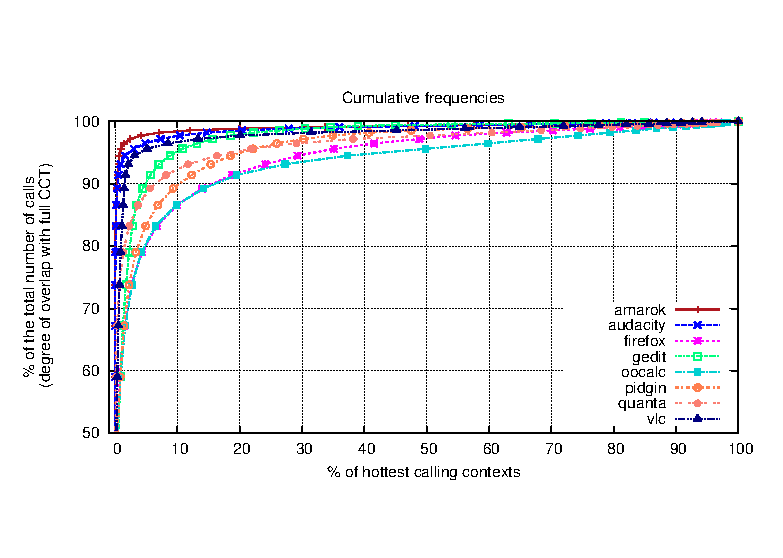
\includegraphics[width=0.95\textwidth]{figures/hcct-skewness/hcct-skewness.eps}
\caption{\protect\label{fig:hcct-skewness} Skewness of calling contexts distribution on a representative subset of applications. For instance, in {\tt oocalc}, 10\% of the hottest calling contexts account for more than 86\% of all routine calls.
}
\end{center}
\end{figure}
\fi

\paragraph*{Contributions.} In this thesis, we introduce a novel run-time data structure, called {\em Hot Calling Context Tree (HCCT)}, that compactly represents all the hot calling contexts encountered during a program's execution, offering an additional intermediate point in the spectrum of data structures for representing interprocedural control flow. The HCCT is a subtree of the CCT that includes only hot nodes and their ancestors, also maintaining estimates of performance metrics (e.g., frequency counts) for hot calling contexts. We cast the problem of identifying the most frequent contexts into a data streaming setting: we show that the HCCT can be computed without storing the exact frequency of all calling contexts, by using fast and space-efficient algorithms for mining frequent items in data streams. These algorithms allow us to distinguish between hot and cold contexts on the fly, and typically provide tight guarantees on the accuracy of returned frequency estimates.

%Context-sensitive profiling provides 
%These algorithms allow us to distinguish between hot and cold context on-the-fly, and we show both theoretically and experimentally that for collected metrics the HCCT achieves a similar precision as the CCT in a space that is several orders of magnitude smaller. We show on prominent benchmarks that our implementation, shipping as a plugin for the \gcc\ compiler, incurs a slowdown competitive with the \gprof\ profiler while collecting much finer-grained profiles.

\subsection{Approach}
\label{ss:hcct-approach}

\paragraph*{Background.} A {\em calling context tree} (CCT) can be used to compactly represent all the calling contexts encountered during the execution of a program. In fact, calling contexts can be straightforwardly mapped to paths in a tree: nodes represent un-returned function calls, and each path from the root to a node $v$ encodes the calling context of the call associated with $v$. As in a tree the path from the root to any other node is always unique, we can also say that each calling context is uniquely represented by a node, which aggregates metrics for identical contexts recurring in the execution. Note that a routine with multiple calling contexts will instead appear more than once in the tree. Slightly extended CCT definitions can be given to bound its depth in the presence of direct recursion, and to distinguish calls that take place at different call sites of the same calling procedure~\cite{Ammons97}.

%The call stack of a program can be mapped to a tree data structure by associating nodes with calls to procedures, so that each path from the root to a node $v$ represents the calling context of the call mapped to $v$. A routine with multiple contexts will appear more than once, but each calling context is represented just once in the CCT and metrics for identical contexts are aggregated.

\paragraph*{Introducing the HCCT.} In order to introduce the hot calling context tree, we have first to define when a context can be called hot. Let $N$ be the number of calling contexts encountered during a program's execution: $N$ equals the number of nodes of the call tree, the sum of the frequency counts of CCT nodes, as well as the number of routine invocations in the execution trace. 

\begin{definition}
A calling context is {\em hot} with respect to a frequency threshold $\phi\in[0,1]$ if and only if the frequency count of its corresponding CCT node is $\geq \lfloor\phi N\rfloor$. 
\end{definition}

\noindent Any calling context that is not hot is said to be {\em cold}. 

\begin{definition}
The {\em Hot Calling Context Tree (HCCT)} is the (unique) subtree of the CCT obtained by pruning all cold nodes that are not ancestors of a hot node.
\end{definition}

\noindent In graph theory, the HCCT corresponds to the Steiner tree of the CCT with hot nodes and the root used as terminals, i.e., to the minimal connected subtree of the CCT spanning hot nodes and the root. The HCCT includes all the hot nodes, and all its leaves are necessarily hot. An example of HCCT is given in \myfigure\ref{fig:hcct-example}(b). 

\ifdefined\noauthorea
\begin{figure}[ht]
\begin{center}
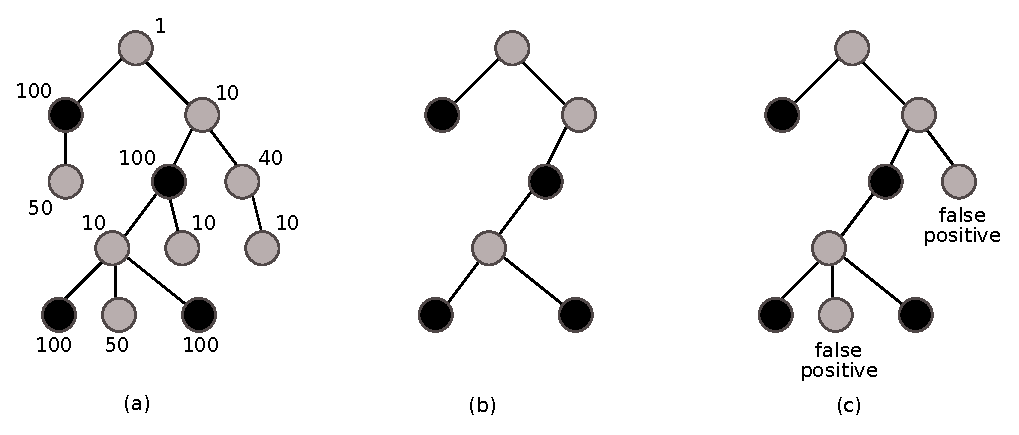
\includegraphics[width=0.95\textwidth]{figures/hcct-example/hcct-example.eps}
\caption{\protect\label{fig:hcct-example} (a) CCT annotated with calling-context frequency counts; (b) HCCT; and (c) $(\phi,\varepsilon)$-HCCT. Hot nodes are black. In this example $N=581$, $\phi=1/10$, and $\varepsilon=1/30$: the approximate HCCT includes all contexts with frequency $\ge\lfloor\phi N\rfloor=58$  and no context with frequency $\le\lfloor(\phi-\varepsilon) N\rfloor=38$.
}
\end{center}
\end{figure}
\fi

\subsubsection*{A Data Streaming Problem}
The execution trace of routine invocations and terminations can be naturally regarded as a stream of items. Each item is a triple containing routine name, call site, and event type (i.e., routine invocation or termination). Figures reported in \mytable\ref{tab:hcct-CCTsize} indicate that, even for complex applications, the number of distinct routines (i.e., the number of nodes of the call graph) is small compared to the stream length (i.e., to the number of nodes of the call tree). Hence, non-contextual profilers -- such as vertex profilers -- can easily collect performance metrics for all the routines using a hash table. This may not be sustainable
%in the case of contextual profiling, when %
for contextual profiling when the number of distinct calling contexts (i.e., the number of CCT nodes) is too large, and hashing would be inefficient. Motivated by the fact that execution traces are typically very long and their items (calling contexts) are taken from a large universe, we cast the problem of identifying the most frequent contexts into a data streaming setting.

In the data streaming computational model, algorithms should be able to perform near-real time analyses on massive data streams, where input data come at a very high rate and cannot be stored entirely due to their huge, possibly unbounded size~\cite{Demetrescu07,Muthukrishnan05}. This line of research has been mainly motivated by networking and database applications: for instance, a relevant IP traffic analysis task consists in monitoring the packet log over a given link in order to estimate how many distinct IP addresses used that link in a given period of time. Space-efficient data streaming algorithms can maintain a compact data structure that is dynamically updated upon arrival of new input data, supporting a variety of application-dependent queries. Approximate answers are allowed when it is impossible to obtain an exact solution using only limited space. Streaming algorithms are therefore designed to optimize space usage and update/query time while guaranteeing high solution quality~\cite{Muthukrishnan05}.

We remark that the practical requirements for the design of effective dynamic analysis tools -- which have to collect and process large amounts of data in nearly real time and with a minimal impact on the running program -- make it natural to look for the connections between these two research areas.

\paragraph*{Finding Frequent Items in a Stream.} The problem of computing the HCCT online can be reduced to the {\em frequent items} (a.k.a. heavy hitters) problem, which has been extensively studied in the data streaming model. Given a frequency threshold $\phi\in[0,1]$ and a stream of length $N$, the problem (in its simplest formulation) is to find all items that appear in the stream at least $\lfloor\phi N\rfloor$ times, i.e., having frequency $\ge\lfloor\phi N\rfloor$. For instance, for $\phi=0.1$ the problem seeks all items that appear in the stream at least $10\%$ of the time. Notice that at most $1/\phi$ items can have frequency larger than $\lfloor\phi N\rfloor$.  It can be proved that any algorithm that outputs an exact solution requires $\Omega(N)$ bits, even using randomization~\cite{Muthukrishnan05}. Note that this lower bound result extends to the problem of computing the HCCT, which cannot be calculated exactly in a space asymptotically smaller than the entire CCT. Hence, researchers have focused on solving an approximate version of the heavy hitters problem~\cite{Muthukrishnan05}:

\begin{definition} 
{\mbox{$(\phi,\varepsilon)$-heavy hitters problem.}} Given two parameters $\phi,\varepsilon\in[0,1]$, with $\varepsilon<\phi$, an algorithm has to return all items with frequency $\ge\lfloor\phi N\rfloor$ and no item with frequency $\le\lfloor(\phi-\varepsilon) N\rfloor$.
\end{definition} 

\noindent In the approximate solution, {\em false negatives} are not allowed, i.e., all frequent items must be returned. Instead, some {\em false positives} can exist, but their actual frequency is guaranteed to be at most $\varepsilon N$--far from the threshold $\lfloor\phi N\rfloor$. For the HCCT construction, we focus on a variant of the problem where, besides returning the heavy hitters, it is necessary to estimate their true frequencies accurately, the stream length $N$ is not known in advance, and all the items in the stream have equal weight.

Counter-based streaming algorithms solve this problem by tracking a subset of items from the input and monitoring counts associated with them. For each new arrival, the algorithms decide whether to store the item or not, and, if so, what count to associate with it. Update times are typically dominated by a small (constant) number of dictionary or heap operations. These algorithms, according to extensive experimental studies~\cite{Cormode08,Manerikar09}, have superior performance with respect to space, running time, and accuracy compared to other classes of algorithms for $(\phi,\varepsilon)$-heavy hitters
%that have been proposed in the literature in the last 15 years.
that have been proposed in the last 15 years.

\subsubsection*{Approximating the HCCT}
Streaming algorithms for mining frequent items can be used to solve a relaxed version of the HCCT construction problem. We thus rely on them to compute an {\em Approximate Hot Calling Context Tree} that we denote by {\em $(\phi,\varepsilon)$-HCCT}, where $\varepsilon<\phi$ controls the degree of approximation:

\begin{definition}
Given a set A of $(\phi,\varepsilon)$-heavy hitters, the {\em $(\phi,\varepsilon)$-HCCT} is the minimal connected subtree of the CCT spanning all the nodes in A and their ancestors.
\end{definition}

\noindent A $(\phi,\varepsilon)$-HCCT contains all hot nodes ({\em true positives}), but may possibly contain some cold nodes without hot descendants ({\em false positives}). The true frequency of these false positives, however, is guaranteed to be at least $\lfloor(\phi-\varepsilon) N\rfloor$. Unlike the HCCT, a $(\phi,\varepsilon)$-HCCT is not uniquely defined, since the set of $(\phi,\varepsilon)$-heavy hitters is not unique: nodes with frequencies smaller than $\lfloor\phi N\rfloor$ and larger than $\lfloor(\phi-\varepsilon) N\rfloor$ may be either in such a set or not depending on the streaming algorithm's decisions.
%depending on the streaming algorithm in use.
On the other hand, the HCCT is always a subtree of any $(\phi,\varepsilon)$-HCCT, as the latter always contains all the hot nodes and their cold ancestors up to the CCT root.

\ifdefined\noauthorea
\begin{figure}[ht]
%\begin{center}
\centering
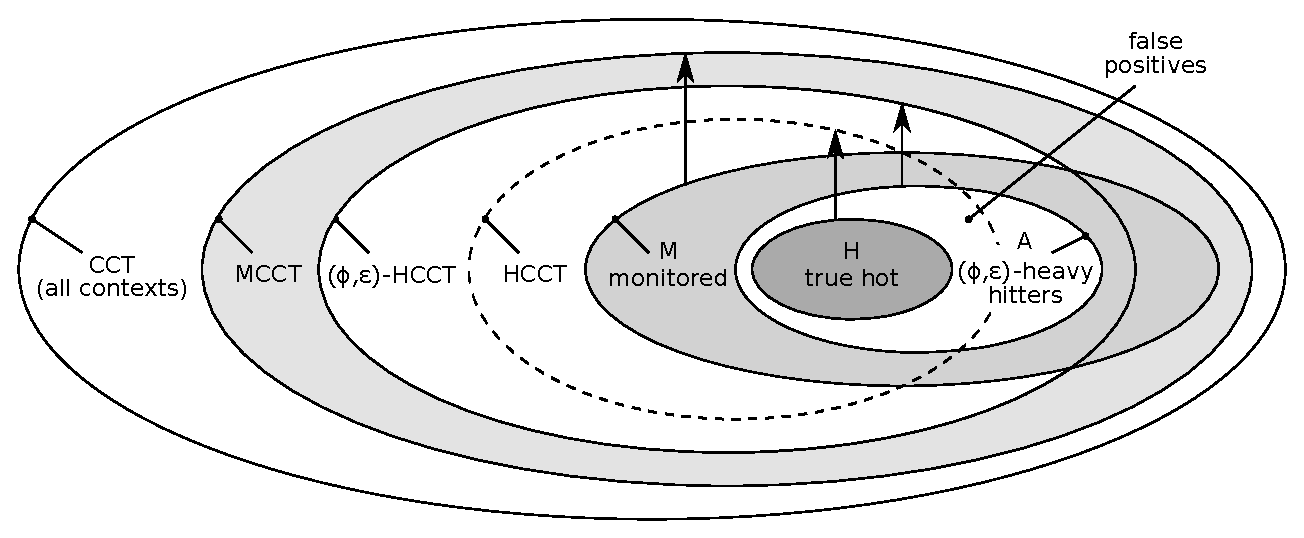
\includegraphics[width=0.95\textwidth]{figures/hcct-venn/hcct-venn.eps}
\caption{\protect\label{fig:hcct-venn} Tree data structures and calling contexts classification. Graphical notation S $\uparrow$ T indicates that T is the minimal subtree of the CCT spanning all nodes in S.
}
%\end{center}
\end{figure}
\fi

\subsection{Algorithms}
\label{ss:hcct-algorithms}

Computing a $(\phi,\varepsilon)$-HCCT online requires extending the canonical CCT construction algorithm with an online pruning strategy, driven by an underlying streaming routine. Constructing a CCT on-the-fly during the execution of a program is rather simple. Let $v$ be a cursor pointer that points to the current context, i.e., to the node corresponding to the calling context of the currently active routine ($v$ is initialized to the CCT root node). At each routine invocation, the algorithm checks whether $v$ has a child associated with the called routine. If this is the case, the existing child is used and its metrics are updated, if needed. Otherwise, a new child of $v$ is added to the CCT. In both cases, the cursor is moved to the callee. Upon routine termination, the cursor is moved back to the parent node in the CCT. This approach can be implemented by either instrumenting every routine call and return, or performing stack-walking when sampling is used to inhibit redundant profiling~\cite{Arnold00,Whaley00,Zhuang06}.

In order to compute the set A of $(\phi,\varepsilon)$-heavy hitters, counter-based streaming algorithms need to monitor a slightly larger set M$\,\supseteq\,$A of elements. Nodes in M$\,\setminus\,$A can be either ancestors of nodes in A and thus already in the $(\phi,\varepsilon)$-HCCT, or nodes not in the $(\phi,\varepsilon)$-HCCT; for the latter category, we have to retain information about their ancestors as well, which might not be in the $(\phi,\varepsilon)$-HCCT. We denote as MCCT the minimal subtree of the CCT spanning all the nodes in M and the CCT root. \myfigure\ref{fig:hcct-venn} graphically illustrates the relationships among all our data structures.

Our $(\phi,\varepsilon)$-HCCT construction algorithm dynamically maintains the MCCT while the underlying streaming routine processes the execution trace and updates M. At query time, the streaming algorithm analyzes M to discard all the elements in M$\,\setminus\,$A: the MCCT is thus pruned appropriately and the $(\phi,\varepsilon)$-HCCT$\,\subseteq\,$MCCT is returned.

\begin{example}
To understand why the heavy hitters and the approximate HCCT are not maintained directly, but derived by pruning M and MCCT, respectively, we discuss a scenario where M is larger than the number of heavy hitters. Consider the following example: the execution trace contains the initial invocation of the {\tt main} function, which in turn invokes once a routine $p$, and $N-2$ times a different routine $q$. Hence, we have three distinct calling contexts: {\tt main}, {\tt main}$\rightarrow${\tt p}, and, {\tt main}$\rightarrow${\tt q}. Assume that $N\ge 8$, $\varepsilon=1/4$, $\phi=1/2$, and that the counter-based streaming subroutine can maintain three counters, one for each calling context. Then, only context {\tt main}$\rightarrow${\tt q} has frequency larger than $\lfloor(\phi-\varepsilon)N\rfloor$ and is a $(\phi,\varepsilon)$-heavy hitter, but -- as we assumed there is room in M for all contexts -- a streaming algorithm can maintain the exact frequencies of both {\tt main}$\rightarrow${\tt p} and {\tt main}$\rightarrow${\tt q}. Since {\tt main}$\rightarrow${\tt p} has frequency 1, it would be an error returning it as a heavy hitter. For this reason, M needs to be post-processed in order to eliminate low-frequency items that may be included when there are more available counters than heavy hitters.
\end{example}

\subsubsection*{Data Structure Operations}
At each function call, the set M of monitored contexts is updated by a counter-based streaming algorithm. When M is changed, the subtree MCCT spanning nodes in M needs to be brought up to date as well. To describe how this happens, we assume that the interface of the streaming algorithm provides two main functions:

%TODO fix alignment
%\begin{enumerate}[align=left,leftmargin=*]
\begin{description}
\item[{\tt update(x,M)}$\rightarrow\,${\tt V}] Given a calling context $x$, update M to reflect the new occurrence of $x$ in the stream (e.g., if $x$ was already monitored in M, its frequency count may be increased by one). This function might return a set V of {\em victim} contexts that were previously monitored in M and are evicted during the update (as a special case, $x$ itself may be considered as a victim if the algorithm chooses not to monitor it).
\item[{\tt query(M)}$\rightarrow\,${\tt A}] Remove low-frequency items from M and return the subset A of $(\phi,\varepsilon)$-heavy hitters (see \myfigure\ref{fig:hcct-venn}).
\end{description}
%\end{enumerate}

\ifauthorea{}{\par\begingroup \parfillskip 0pt \relax}
\noindent As with the CCT, during the construction of the MCCT we maintain a cursor pointer that points to the current calling context, creating a new node if the current context $x$ is not already represented in the tree. Additionally, we prune the MCCT according to the victim contexts returned by the streaming {\tt update} operation (these contexts are no longer monitored in M). The pseudocode of the pruning algorithm is given in \myalgorithm\ref{alg:hcct-update}. Since the tree must remain connected, victims can be removed from
the MCCT only if they are leaves. Moreover, removing a victim might expose a path of unmonitored ancestors that no longer have descendants in M: these nodes 
\ifauthorea{}{\par\endgroup}
\ifdefined\noauthorea

\begin{figure}[h!]
\IncMargin{2em}
\begin{algorithm}[H]
\LinesNumbered
\SetAlgoNoLine
\SetNlSkip{1.5em} 
\Indm\Indmm
\nonl\hrulefill\\
\KwIn{M; MCCT; node $x$ to be pruned.}
\KwOut{Pruned MCCT.}
\vspace{-2mm}\hrulefill\\
\Indp\Indpp
$V$ $\gets$ {\tt update}(x, M);\\
\ForEach{context $v\in V\,\backslash \{x\}$}{
    \While{$(v$ is a leaf in MCCT$)$ $\wedge$ $(v\not\in$ M$)$}{
        remove $v$ from MCCT\\
        $v$ $\gets$ parent$(v)$
    }
}
\vspace{-2mm}
\Indm\Indmm
\nonl\hrulefill\vspace{1mm}\\
\DecMargin{2em}
\caption{\label{alg:hcct-update} Online pruning algorithm for MCCT construction.}
\end{algorithm}
\end{figure}


\noindent
\fi
are pruned as well. The node for the current context $x$ is never removed from the MCCT, even if the context is not necessarily monitored in M. This guarantees that no node in the path from the tree root to $x$ will be removed: these nodes have at least $x$ as a descendant and the leaf test (line 3 in \myalgorithm\ref{alg:hcct-update}) will always fail. %Also, it simplifies the MCCT construction when [...]

\noindent
A similar pruning strategy can be used to compute the $(\phi,\varepsilon)$-HCCT from the MCCT. The streaming {\tt query} operation is first invoked on M, returning the support A of the $(\phi,\varepsilon)$-HCCT. All MCCT nodes that have no descendant in A are then removed, following bottom-up path traversals as in the prune operation.

\ifx\noauthorea\undefined
\begin{figure}[ht]
\caption{\label{alg:hcct-update} Online pruning algorithm for MCCT construction.}
\begin{small}
\begin{minipage}{0.9\textwidth}
\hrulefill\\
\textbf{Input}: {MCCT; node $x$ to be pruned.}\\
\textbf{Output}: {Pruned MCCT.}

\vspace{-1mm}
\hrulefill\\
1. ~~ $V$ $\gets$ {\tt update}(x, M);\\
2. ~~ \textbf{foreach} context $v\in V\,\backslash \{x\}$ \textbf{do}\\
3. ~~ ~~~~ \textbf{while} $(v$ is a leaf in MCCT$)$ $\wedge$ $(v\not\in$ M$)$ \textbf{do}\\
4. ~~ ~~~~ ~~~~ remove $v$ from MCCT\\
5. ~~ ~~~~ ~~~~ $v$ $\gets$ parent$(v)$\\
6. ~~ ~~~~ \textbf{end}\\
7. ~~ \textbf{end}

\vspace{-1mm}
\hrulefill
\vspace{-2mm}
\end{minipage}
\end{small}
\end{figure}
\fi

\ifauthorea{\newline}{}
\subsubsection*{Choosing a Streaming Algorithm}
{\em \spacesaving}~\cite{Metwally06} is a deterministic, counter-based algorithm for finding the heavy hitters and the top-$k$ elements~\cite{Charikar02} in data streams. The algorithm is memory-efficient, as its space requirements are within a constant factor of the lower bound for counter-based algorithms solving the $(\phi,\varepsilon)$-heavy hitters problem. Additionally, \spacesaving\ provides tight error guarantees on maintained frequency estimates. In an earlier work~\cite{Delia11}, we presented a thorough
experimental evaluation of the {\em Lossy Counting}~\cite{Manku02} algorithm, resulting in similar accuracy but higher running time and memory usage compared to \spacesaving. Experimental studies~\cite{Cormode08,Manerikar09} also show that \spacesaving\ outperforms other counter-based algorithms across a wide range of data sets and parameters. For all these reasons, in the remainder of this thesis we will focus on the \spacesaving\ algorithm only.

%Sticky Sampling~\cite{Manku02} is probabilistic: it fails to produce the correct answer with a minuscole probability, say $\delta$, and uses at most $\frac{2}{\varepsilon} \log(\phi^{-1}\delta^{-1})$ entries in its data structure. Lossy Counting~\cite{Manku02} is deterministic and maintains up to $\frac{1}{\varepsilon}\log(\varepsilon N)$ entries.

\spacesaving\ monitors a set of $1/\varepsilon=|M|$ pairs of the form $(item, count)$, initialized by the first $1/\varepsilon$ distinct items and their exact counts. After the init phase, when a context $c$ is observed in the stream the {\tt update} operation works as follows: 

\begin{enumerate}[parsep=0pt,topsep=3pt]
\item if $c$ is monitored, the corresponding counter is incremented; 
\item if $c$ is not monitored, the $(item, count)$ pair with the smallest count is chosen as a victim and has its item replaced with $c$ and its count incremented.
\end{enumerate}

\noindent It can be shown that the minimum counter value $min$ among monitored items is never greater than $\varepsilon N$, and that the $count$ maintained for an item is an overestimation of its true frequency by at most $min$. This overestimation derives from the initial assignment to $count$ from the evicted pair. Observe that items that are stored early in the stream and never removed will have very accurate frequency estimates.

The update time is bounded by the dictionary operation of checking whether an item is monitored, and by the operations of finding and maintaining the item with minimum count. In our setting, we can avoid the dictionary operation by maintaining a flag for each tree node, which can directly be accessed for the current context using the cursor pointer to the MCCT.

%A {\tt query} operation is answered by returning entries in M such that $count \geq \lfloor\phi N\rfloor$.
\spacesaving\ answers {\tt query} operations by simply returning entries in M such that $count \geq \lfloor\phi N\rfloor$; associated frequency estimates are guaranteed to be at most $\varepsilon N$--far from actual frequencies.

\paragraph*{Engineering \spacesaving.} In~\cite{Metwally06}, the authors present an implementation of \spacesaving\ based on the {\em Stream-Summary} data structure, which is essentially an ordered bucket list where each bucket points to a list of items with the same count, and buckets are ordered by increasing count values.

\noindent We devise a more efficient variant based on a lazy priority queue that uses an unordered array M of size $1/\varepsilon$, where each entry points to an MCCT node. The queue supports two operations, {\tt find-min} and {\tt increment}, which return the item with minimum count and increment a counter, respectively.

We (lazily) maintain the value {\tt min} of the minimum counter and the smallest index {\tt min-idx} of an array entry that points to a monitored node with counter equal to {\tt min}. The {\tt increment} operation does not change M, since counters can be stored directly inside MCCT nodes. However, {\tt min} and {\tt min-idx} may become temporarily out of date after an {\tt increment}: this is why we call the approach lazy. The {\tt find-min} operation described in \myalgorithm\ref{alg:hcct-findMin} restores the invariant property on {\tt min} and {\tt min-idx}: it finds the next index in M with counter equal to {\tt min}. If such an index does not exist, it completely rescans M in order to find a new {\tt min} value and its corresponding {\tt min-idx}.

\ifdefined\noauthorea
\begin{figure}[h!]
\IncMargin{2em}
\begin{algorithm}[H]
\LinesNumbered
\SetAlgoNoLine
\SetNlSkip{1.5em} 
\Indm\Indmm
\nonl\hrulefill\\
\KwIn{M, {\tt min}, and {\tt min-idx}.}
\KwOut{Min value in the lazy priority queue.}
\vspace{-2mm}\hrulefill\\
\Indp\Indpp
\While{$(M[$min-idx$] \neq$ min $)\,\wedge\,($ min-idx $\leq M)$}{
    min-idx $\gets$ min-idx $+ 1$}
\If{min-idx $> M$}{
    min $\gets$ minimum in $M$ \\
    min-idx $\gets$ smallest index $j$ s.t. $M[j] =$ min \\
}
\Return{min}\\
\vspace{-2mm}
\Indm\Indmm
\nonl\hrulefill\vspace{1mm}\\
\DecMargin{3.5em}
\caption{\label{alg:hcct-findMin} {\tt find-min} operation used in {\em lazy} Space Saving.}
\IncMargin{1.5em}
\end{algorithm}
\end{figure}

\else
\begin{figure}[ht]
\caption{\label{alg:hcct-findMin} {\tt find-min} operation used in {\em lazy} Space Saving.}
\begin{small}
\begin{minipage}{0.9\textwidth}
\hrulefill\\
\textbf{Input}: {M, {\tt min}, and {\tt min-idx}.}\\
\textbf{Output}: {Min value in the lazy priority queue.}

\vspace{-1mm}
\hrulefill\\
1. ~~ \textbf{while} $(M[$min-idx$] \neq$ min $)\,\wedge\,($ min-idx $\leq M)$ \textbf{do}\\
2. ~~ ~~~~ min-idx $\gets$ min-idx $+ 1$\\
3. ~~ \textbf{end}\\
4. ~~ \textbf{if} min-idx $> M$ \textbf{then}\\
5. ~~ ~~~~ min $\gets$ minimum in $M$\\
6. ~~ ~~~~ min-idx $\gets$ smallest index $j$ s.t. $M[j] =$ min\\
7. ~~ \textbf{end}\\
8. ~~ \textbf{return} min

\vspace{-1mm}
\hrulefill
\vspace{-2mm}
\end{minipage}
\end{small}
\end{figure}
\fi

\ifauthorea{\newline}{}
\noindent By proving that {\tt find-min} requires constant amortized time, we show that an {\tt update} operation can be performed in constant time during the MCCT construction:
\begin{theorem}
%\vspace{-2mm}
After a {\tt find-min} query, the lazy priority queue correctly returns the minimum counter value in O(1) amortized time.
\end{theorem}
\begin{myproof} Counters are never decremented. Hence, at any time, if a monitored item with counter equal to {\tt min} exists, it must be found in a position larger than or equal to {\tt min-idx}. This yields correctness.

To analyze the running time, let $\Delta$ be the value of {\tt min} after $k$ {\tt find-min} and {\tt increment} operations. Since there are $|M|$ counters $\ge\Delta$, counters are initialized to $0$, and each {\tt increment} operation adds 1 to the value of a single counter, it must be $k\ge |M|\cdot\Delta$. For each distinct value assumed by {\tt min}, the array is scanned twice. We therefore have at most $2\cdot\Delta$ array scans each of length $|M|$, and the total cost of {\tt find-min} operations throughout the whole sequence of operations is upper bounded by $2\cdot|M|\cdot\Delta$. It follows that the amortized cost is $(2\cdot|M|\cdot\Delta)/k\leq 2$.
\end{myproof}

\noindent Using a simple amortized analysis argument, it can be shown that the running time of \myalgorithm\ref{alg:hcct-update} for tree pruning is constant as well.

%\mynote{Write an informal proof for pruning?}

\subsection{Discussion}

Compared to the standard approach of maintaining the entire CCT, our solution requires storing the heavy hitters data structure M and the subtree MCCT spanning nodes in M. The space required by M depends on the specific streaming algorithm that is used as a subroutine and on the value chosen for the error threshold $\varepsilon$. For \spacesaving\, this space is proportional to $1/\varepsilon$ and can be customized by appropriately choosing $\varepsilon$, e.g., according to the desired accuracy or to the amount of memory available for profiling. Such a choice appears to be crucial for the effectiveness of our approach: smaller values of $\varepsilon$ guarantee more accurate results (i.e., fewer false positives and more precise counters), but imply a larger memory footprint. In \mysection\ref{ss:hcct-eval} we will see that the high skewness of context frequency distribution guarantees the existence of very convenient trade-offs between accuracy and space in the analysis of real-world programs.

The MCCT consists of nodes corresponding to contexts monitored in M and all their ancestors, which may be cold contexts without a corresponding entry in M. Hence, the space required by the MCCT dominates the space required by M. The number of cold ancestors is difficult to analyze theoretically: it depends on properties of the execution trace and on the structure of the CCT. In \mysection\ref{ss:hcct-accuracy} we will see that in practice this amount is negligible compared to the size of M.

Updates of the MCCT can be performed very quickly. We propose an engineered implementation of \spacesaving\ that hinges upon very simple and cache-efficient data structures, and might be of independent interest.

Unlike previous approaches such as, e.g., adaptive bursting~\cite{Zhuang06}, the MCCT adapts automatically to the case where the hot calling contexts vary over time, and new calling patterns are not likely to be lost. Contexts that are growing more popular are added to the tree as they become more frequent, while contexts that lose their popularity are gradually replaced by hotter contexts and are finally discarded. This guarantees that heavy hitters queries can be issued at any point in time, and will always be able to return the set of hot contexts up to that time.

%Our data streaming-based approach is orthogonal to previous techniques and can be integrated, e.g., with sampled stack-walking~\cite{Arnold00,Whaley00} or with more recent techniques such as static and adaptive bursting~\cite{Zhuang06}. We will show an example of integration with static bursting, which results in faster running times without substantially affecting accuracy.

%In addition to frequency counts, it can be extended to support arbitrary performance metrics (e.g., execution time, cache misses, instruction stalls), exploiting the ability of some streaming algorithms to mine heavy hitters in weighted item sets.

\subsection{Comparison with Related Work}

CCTs have been introduced in~\cite{Ammons97} as a practical data structure to associate performance metrics with paths through a program's call graph: Ammons, Ball, and Larus suggest to build a CCT by instrumenting procedure code and to compute metrics by exploiting hardware counters available in modern processors. It has been later observed, however, that exhaustive instrumentation can incur large slowdowns.

\paragraph*{Reducing Overhead.} To reduce the overhead from instrumentation, in~\cite{Bernat07} the authors generate path profiles including only methods of interest, while statistical profilers~\cite{Arnold00,Froyd05,Hall93,Whaley00} attribute metrics to calling contexts through periodic sampling of the call stack. For call-intensive programs, sample-driven stack-walking can be orders of magnitude faster than exhaustive instrumentation, but may incur significant loss of accuracy with respect to the complete CCT: sampling guarantees neither high coverage~\cite{Bond07} nor accuracy of performance metrics~\cite{Zhuang06}, and its results may be highly inconsistent in different executions.

\noindent A variety of works explores the combination of sampling with bursting~\cite{Arnold01,Hirzel01,Zhuang06}. Most recently, Zhuang {\em et al.} suggest to perform stack-walking followed by a burst during which the profiler traces every routine call and return~\cite{Zhuang06}: experiments show that adaptive bursting can yield very accurate results. In~\cite{Serrano09}, the profiler infrequently collects small call traces that are merged afterwards to build large calling context trees: ambiguities might emerge during this process, and the lack of information about where the partial CCTs should be merged to does not allow a univocal reconstruction of the entire CCT.

The main goal of all these works is to reduce profiling overhead without incurring significant loss of accuracy. Our approach is orthogonal to this line of research and regards space efficiency as an additional resource optimization criterion besides profile accuracy and time efficiency. When the purpose of profiling is to identify hot contexts, exhaustive instrumentation, sampling, and bursting might all be combined with our approach and benefit of our space reduction technique. In \mysection\ref{ss:hcct-implementation} we present an integration of our technique with static bursting~\cite{Zhuang06}, which results in faster running times without substantially affecting accuracy.

\paragraph*{Reducing Space.} A few previous works have addressed techniques to reduce profile data (or at least the amount of data presented to the user) in context-sensitive profiling. Incremental call-path profiling lets the user choose a subset of routines to be analyzed~\cite{Bernat07}. Call path refinement helps users focus the attention on performance bottlenecks by limiting and aggregating the information revealed to the user~\cite{Hall95}. These works are quite different in spirit from our approach, where only hot contexts are profiled and identified automatically during program's execution.

Probabilistic calling contexts have been introduced as an extremely compact representation (just a 32-bit value per context), especially useful for tasks such as residual testing, statistical bug isolation, and anomaly-based intrusion detection~\cite{Bond07}. Bond and McKinley target applications where coverage of both hot and cold contexts is necessary, but their inspection is unnecessary. This is not the case in performance analysis, where identifying and understanding a few hot contexts is typically sufficient to guide code optimization. Hence, although sharing with~\cite{Bond07} the common goal of space reduction, our approach targets a rather different application context.

Somner et al. proposed a technique called {\em Precise Calling Context Encoding} (PCCE) that encodes acyclic paths in the call graph of a program into one number, while recursive call paths are divided into acyclic subsequences and encoded independently~\cite{Sumner10,Sumner12}. Different calling contexts are guaranteed to have different IDs that can be faithfully decoded, and experiments on a prototype implementation for C programs show negligible overhead. However, PCCE would not work in the presence of virtual methods and dynamic class loading in object-oriented languages, and the encoding scheme shows scalability problems when handling large-scale software~\cite{Bond10,Zeng14}. These limitations, which are absent from our solution, have been recently addressed in~\cite{Zeng14}, and it would be interesting to investigate whether their approach can be extended to collect performance metrics and in turn filter the collected data on-the-fly using a data streaming approach as we do in this thesis.

%\paragraph*{Other Related Work} In a recent work~\cite{Huang13}, a novel data structure is proposed to avoid the node lookup operation in dynamic bug detectors. A new node is instead allocated for each context, and the costs of memory allocation are mitigated by extending the garbage collector not only to collect unused nodes, but also to merge duplicate nodes lazily.
% Ausiello's OOPSLA'12 paper (k-calling context)

\ifdefined\noauthorea
\section{Intraprocedural Profiling}

{\em Path profiling} is a powerful {\em intraprocedural} methodology for identifying performance bottlenecks in a program, and has received considerable attention in the last 15 years for its practical relevance. The well-known Ball and Larus numbering algorithm~\cite{Ball96} can efficiently encode {\em acyclic} paths that are taken across the control-flow graph of a function. Previous attempts to extend it to {\em cyclic} paths, as spanning multiple loop iterations, to capture more optimization opportunities, are based on rather complex algorithms that incur severe performance overheads even for short cyclic paths. In this thesis we present a new, data-structure based approach to {\em multi-iteration} path profiling built on top of the original Ball-Larus numbering technique. Starting from the observation that a cyclic path can be described as a concatenation of Ball-Larus acyclic paths, we show how to accurately profile all executed paths obtained as a concatenation of up to $k$ Ball-Larus paths, where $k$ is a user-defined parameter.

%{\em Path profiling} is a powerful {\em intraprocedural} methodology for identifying performance bottlenecks in a program, and has received considerable attention in the last 15 years for its practical relevance. The well-known Ball and Larus algorithm~\cite{Ball96} for {\em intraprocedural} path profiling can efficiently encode {\em acyclic} paths that are taken across the control-flow graph of a function. Previous attempts to extend it to encode {\em cyclic} paths, and thus to span multiple loop iterations in order to capture more optimization opportunities, are based on rather complex algorithms that incur severe performance overheads even for short cyclic paths. In this thesis we present a new, data-structure based approach to {\em multi-iteration} path profiling built on top of the original Ball-Larus numbering technique. Starting from the observation that any cyclic path can be described as a concatenation of Ball-Larus acyclic paths, we show how to accurately profile all executed paths obtained as a concatenation of up to $k$ Ball-Larus paths, where $k$ is a user-defined parameter.

%We provide examples showing that this method can reveal optimization opportunities that acyclic-path profiling would miss, and we present an extensive experimental investigation on a large variety of Java benchmarks in the Jikes RVM. Experiments show that our approach can be even faster than a hash table-based implementation of the Ball-Larus algorithm due to fewer operations on smaller tables, producing compact representations of cyclic paths even for large values of $k$.

\subsection{Motivation and Contributions}

Path profiling associates performance metrics, usually frequency counters, to paths taken in the control flow graph of a routine. Identifying the hottest paths can direct optimizations to portions of the code where most resources are consumed, often yielding significant speedups. For instance, trace scheduling can improve performance by increasing instruction-level parallelism along frequently executed paths~\cite{Fisher81,Young98}. Although basic block and edge profiles are inexpensive and widely available, they do not always correctly predict frequencies of overlapping paths. 

The seminal paper by Ball and Larus~\cite{Ball96} introduced a simple and elegant path profiling technique. The main idea was to implicitly number all possible acyclic paths in the control flow graph so that each path is associated with a unique compact path identifier (ID). The authors showed that path IDs can be efficiently generated at runtime and can be used to update a table of frequency counters. Although in general the number of acyclic paths may grow exponentially with the graph size, in typical control flow graphs this number is usually small enough to fit in current machine word-sizes, making this approach very effective in practice.

While the original Ball-Larus approach was restricted to acyclic paths obtained by cutting paths at loop back edges, profiling paths that span consecutive loop iterations is a desirable, yet difficult, task that can yield better optimization opportunities. Consider, for instance, the problem of eliminating redundant executions of instructions, such as loads and stores~\cite{Bodik99}, conditional jumps~\cite{Bodik97}, expressions~\cite{Bodik98,Bodik04}, and array bounds checks~\cite{Bodik00}. A typical situation is that the same instruction is redundantly executed at each loop iteration, which is particularly common for arithmetic expressions and load operations~\cite{Bodik04,Bodik99}. To identify such redundancies, paths that extend across loop back edges need to be profiled. Another application is trace scheduling~\cite{Young98}: if a frequently executed cyclic path is found, compilers may unroll the loop and perform trace scheduling on the unrolled portion of code. Tallam {\em et al.}~\cite{Tallam04} provide a comprehensive discussion of the benefits of multi-iteration path profiling.

Different authors have proposed techniques to profile cyclic paths by modifying the original Ball-Larus path numbering scheme in order to identify paths that extend across multiple loop iterations~\cite{Tallam04,Roy09,Li12}. Unfortunately, all known solutions require rather complex algorithms that incur severe performance overheads even for short cyclic paths, leaving the interesting open question of finding simpler and more efficient alternative methods.

\paragraph*{Contributions.}

\subsection{Approach}

\subsection{Algorithms}

%\subsection{Implementation}

\subsection{Comparison with Related Work}

\subsection{Discussion}
\fi
\chapter{Continuous Program Optimization Techniques}
\label{ch:continuous}

\section{Implementing On-Stack Replacement in LLVM}

\section{On-Stack Replacement in the Presence of Compiler Optimizations}
% !TEX root = thesis.tex

\chapter{Experimental Evaluation}
\label{ch:experiments}

In this chapter we illustrate experimental studies that we have performed for the techniques described in \mychapter\ref{ch:profiling,ch:continuous}, which have been implemented in production systems and evaluated against prominent benchmarks.  

%typically evaluated against industry-strength benchmarks. For performance metrics, reported figures have been obtained by performing multiple runs in a Linux system with negligible background activity, and we also show confidence intervals stated at $95\%$ confidence level where possible.

In the first part of the chapter, we evaluate our space-efficient inter-procedural technique for context-sensitive profiling. In our analysis, we take into account a large collection of popular interactive Linux applications and industrial-strength benchmarks. Results collected for a number of accuracy and space usage metrics reinforce the theoretical prediction that the Hot Calling Context Tree (HCCT) achieves a similar precision as the CCT in a several orders of magnitude smaller, and roughly proportional to the number of hot contexts. Our implementation is cast in a full-fledged infrastructure that we developed for profiling multi-threaded Linux C/C++ applications, and ships as a plugin for the GNU Compiler Collection. We also discuss how we integrated our technique with static bursting, resulting in faster running times without substantially affecting accuracy: we incur a slowdown competitive with the \gprof\ call-graph profiler while collecting finer-grained program profiles. 

In the second part, we discuss an implementation in Jikes RVM of our intra-procedural technique for multi-iteration path profiling. We present a broad experimental study on a large suite of prominent Java benchmarks, showing that our profiler can collect profiles that would have been too costly to gather using previous multi-iteration techniques. The key to the efficiency of our approach is to replace costly hash table accesses, which are  required by the Ball-Larus algorithm to maintain path counters for larger programs, with substantially faster operations on trees. We then study structural properties of path profiles that span multiple iterations for several representative benchmarks, and discuss memory footprints of the \ksf\ and \kipf\ data structures for increasing values of $k$.

Finally, we present an extensive experimental evaluation of our on-stack replacement (OSR) techniques for continuous program optimization. We first analyze the performance of \osrkit\ in the \tinyvm\ proof-of-concept virtual machine that we developed in LLVM. Our goal is to address a number of typical concerns of VM builders, measuring, e.g., the impact of having an OSR point in a hot code portion, and the actual cost of performing an OSR transition. We then present an LLVM implementation of the techniques for automatically constructing OSR mapping described in \mysection\ref{ss:osr-mapping-algorithms}, evaluating the fraction of program locations where they allow OSR to be efficiently fired in prominent benchmarks. Our experiments suggest that bidirectional OSR transitions between rather different program versions can be supported almost everywhere in the code under several classic optimizations.

\ifdefined \noauthorea
\section{HCCT Construction and Accuracy}

In this section, we present an extensive experimental study of our data streaming-based methodology for context-sensitive profiling. We implemented several variants of context-sensitive profilers and we analyzed their performance and the accuracy of the produced $(\phi,\varepsilon)$-HCCT with respect to a number of metrics and using many different parameter settings. Besides the exhaustive approach, where each routine call and return is instrumented, we integrate our solution with previous techniques aimed at reducing time overhead: we focus in particular on static bursting~\cite{Zhuang06}, which offers convenient time-accuracy tradeoffs. The experimental analysis not only confirms, but reinforces the theoretical prediction: the $(\phi,\varepsilon)$-HCCT represents the hot portions of the full CCT very well using only an extremely small percentage of the space required by the entire CCT: all the hottest calling contexts are always identified correctly, their counters are very accurate, and the number of false positives is rather small. With bursting, the running time overhead can be kept under control without affecting accuracy in a substantial way.

\subsection{Implementation}

\paragraph*{Compiler Plugin.} The \gcc\ compiler provides an instrumentation infrastructure to emit calls to analysis routines at the beginning and at the end of each function, passing as arguments the address of the current function and its calling site. On top of these two primitives, we have built a full-fledged infrastructure for context sensitive profiling of multi-threaded Linux C/C++ applications that ships as a plugin\footnote{Source code and documentation are available at: \texttt{https://github.com/dcdelia/hcct}} for the GNU Compiler Collection.

Our plugin provides native support for techniques aimed at reducing runtime overhead, such as sampling and bursting, and does not require modifications to the existing {\tt gcc} installation or to the program to be analyzed (except for its {\tt Makefile}). When a program is compiled, instrumentation is injected into the code by the compiler and the executable is eventually linked against a generic profiling library named {\tt libhcct}. When a user wants to analyze the behavior of an instrumented program, it is possible to switch between different techniques -- including the canonical CCT construction -- or parameter settings with no need to further recompile the code.

\paragraph*{Data Structures.} We use a first-child, next-sibling representation for calling context tree nodes. Each MCCT node also contains a pointer to its parent, the routine ID, the call site, and the performance metric. The first-child, next-sibling representation is space-efficient and still guarantees that the children of each node can be explored in time proportional to their number. According to our experiments with several benchmarks, the average number of scanned children is a small constant around 2-3, so this representation turns out to be convenient also for checking whether a routine ID already appears among the children of a node. The parent field, which is needed to perform tree pruning efficiently (see \myalgorithm\ref{alg:hcct-update} in \mysection\ref{ss:hcct-algorithms}), is not required in CCT nodes. As a routine ID, we simply use the routine address. Overall, CCT and MCCT nodes require 20 and 24 bytes, respectively, on 32 bit architectures. Using a simple bit packing technique~\cite{Standish80}, we also encode in one of the pointer fields a Boolean flag that tells if the calling context associated with the node is monitored in the streaming data structure M, without increasing the number of bytes per node. To improve time and space efficiency, we allocate nodes through a custom, page-based allocator, which maintains blocks of fixed size. Any additional algorithm-specific information needed to maintain the heavy hitters is stored as trailing fields within MCCT nodes.

\paragraph*{Integration with Static Bursting.} Static bursting~\cite{Zhuang06} is a profiling technique that combines the advantages of sampling-based and exhausting profiling mechanisms. As in sampling-based solutions, a bursting profiler lets a program run unhindered between sampling points, and performs stack walking to determine the current calling context when a sampling point is reached. Rather than incrementing the counter for the corresponding node (which may not reflect an actual function call and thus drive to misleading results), a bursting profiler performs exhaustive instrumentation on the sequence (i.e.,  burst) of call/return events collected in an interval whose length we refer to as {\em burst length}. Further refinement of static bursting are possible, e.g., analysis overhead can be further reduced by selectively disabling bursts for previously sampled calling-contexts and then probabilistically re-enabling them~\cite{Zhuang06}. In our setting, driven by the shadow stack maintained by the profiling infrastructure, we update our cursor pointer by walking down the tree from its root. Missing nodes are initialized and added to the tree during the walk. The execution stream we observe is thus partitioned into bursts and sequences that are transparent to profiling.

\paragraph*{Other Software.} As part of our infrastructure, we have developed two additional pieces of software that might be of independent interest: a library for resolving addresses to symbols, and a set of tools for the analysis and comparison of CCTs from distinct executions. In general, even for deterministic benchmarks it might not be trivial to line up nodes from two executions, as due to technical aspects such as address space randomization and dynamic loading of libraries program addresses can change. In some cases it is not always possible to resolve addresses offline up to a source-file line-number granularity, but the available information is only partial (e.g., we know only the source file where the method is defined). If this happens for two or more sibling nodes that have identical frequency counters, lining them up with tree nodes from another execution requires a similarity analysis of their spanned subtrees. We observed similar scenarios frequently in our experiments, both for hot and cold calling contexts. Since spanned subtrees for CCT nodes can be large, rapid and accurate heuristics are required to summarize the subtrees and compute their similarity; accuracy of heuristics is even more crucial when comparing a CCT with a HCCT, as spanned subtrees in the latter might have been partially or entirely pruned. Using combinatorial techniques and ad-hoc heuristics based on topological properties of the trees, we were able to quickly (i.e., in a few minutes) reconstruct for all our experiments a full and accurate mapping between pairs of different trees.

\subsection{Experimental Setup}

In this section we present the details of our experimental methodology, focusing on benchmarks and accuracy metrics, and we describe how the parameters of the streaming algorithms can be tuned.

\subsubsection*{Benchmarks}
Tests were performed on a variety of large-scale Linux applications and on a set benchmarks drawn from the {\tt Phoronix PTS} and the {\tt SPEC CPU2006} test suites. To ensure deterministic replay of the execution of the interactive applications, we used the PIN dynamic instrumentation framework~\cite{Luk05} to record timestamped execution traces for typical usage sessions of appoximately fifteen minutes.

Interactive applications include graphics programs ({\tt inkscape} and {\tt gimp}), a hexadecimal file viewer ({\tt ghex2}), audio players/editors ({\tt amarok} and {\tt audacity}), an archiver ({\tt ark}), an Internet browser ({\tt firefox}), an HTML editor ({\tt quanta}), a chat program ({\tt pidgin}), the OpenOffice suite for word processing ({\tt oowriter}), spreadsheets ({\tt oocalc}), and drawing ({\tt ooimpress}).

Non-interactive benchmarks include a cryptographic library ({\tt botan}), a 2D graphics library ({\tt cairo-perf-trace}), advanced chess engines ({\tt crafty} and {\tt sjeng}), the Connect Four ({\tt fhourstones}) and Go ({\tt gobmk}) games, and two 3D games run in demo mode (PlanetPenguin Racer in the {\tt ice-labyrinth} and {\tt mount-herring} scenarios, and SuperTuxKart on the {\tt overworld} and {\tt scotland} tracks).

Statistical information about test sets are reported in \mytable\ref{tab:hcct-CCTsize}\ifauthorea{}{ (page~\pageref{tab:hcct-CCTsize})}: even short sessions result in CCTs consisting of tens of millions of calling contexts, whereas the call graph has only a few thousand nodes. We also observe that the number of distinct call sites is roughly one order of magnitude larger than the call graph.

\subsubsection*{Metrics}
Besides memory usage and time consumption of our profiler, we test the accuracy of the $(\phi,\varepsilon)$-HCCT according to a variety of metrics.

\begin{enumerate}
\item Degree of overlap~\cite{Arnold01,Arnold00,Zhuang06} measures the completeness of the $(\phi,\varepsilon)$-HCCT with respect to the full CCT:
\begin{small}
$$overlap((\phi,\varepsilon){\mbox{-HCCT,\,CCT}})=\frac{1}{N}\sum_{\mbox{\footnotesize{arcs}}~e\in (\phi,\varepsilon)\mbox{\tiny -HCCT}}w(e)$$\\
\end{small}
where $N$ is the total number of routine activations (corresponding to the CCT total weight) and $w(e)$ is the true frequency of the target node of arc $e$ in the CCT.

\item Hot edge coverage~\cite{Zhuang06} measures the percentage of CCT hot edges covered by the $(\phi,\varepsilon)$-HCCT, using an edge-weight threshold $\tau\in [0,1]$ to determine hotness. Since $(\phi,\varepsilon)$-HCCT$\subseteq$CCT, hot edge coverage can be defined as follows:
\begin{small}
$$\hspace{-0mm}cover((\phi,\varepsilon){\mbox{-HCCT,\,CCT}},\tau)=\frac{|\{e\in(\phi,\varepsilon){\mbox{-HCCT:}}\,w(e)\ge\tau \cdot w_{max}\}|}{|\{e\in\mbox{CCT:}\,w(e)\ge\tau \cdot w_{max}\}|}$$\\
\end{small}
where $w_{max}$ is the weight of the hottest CCT arc.

\item Maximum hotness of uncovered calling contexts, where a context is uncovered if is not included in the $(\phi,\varepsilon)$-HCCT:
\begin{small}
$$maxUncov((\phi,\varepsilon){\mbox{-HCCT,\,CCT}})=\max_{e\in\mbox{\tiny CCT}\setminus(\phi,\varepsilon){\mbox{\tiny -HCCT}}}\frac{w(e)}{w_{max}}\times 100$$\\
\end{small}
Average hotness of uncovered contexts is defined similarly.

\item Number of false positives, i.e., $|A\setminus H|$: the smaller this number, the better the $(\phi,\varepsilon){\mbox{-HCCT}}$ approximates the exact HCCT obtained from CCT pruning.

\item Maximum counter error, i.e., maximum error in the frequency counters of $(\phi,\varepsilon)$-HCCT nodes with respect to their true value in the full CCT:
\begin{small}
$$maxError((\phi,\varepsilon){\mbox{-HCCT}})=\max_{e\in(\phi,\varepsilon){\mbox{\tiny -HCCT}}}\frac{|w(e)-\widetilde{w}(e)|}{w(e)}\times 100$$\\
\end{small}
where $w(e)$ and $\widetilde{w}(e)$ are the true and the estimated frequency of context $e$, respectively. Average counter error is defined similarly.
\end{enumerate}

\noindent We remark that an accurate solution should maximize (1) and (2), and minimize the remaining metrics.

\subsubsection*{Parameter Tuning}

Before describing our experimental findings, we discuss how to choose parameters $\phi$ and $\varepsilon$ to be provided as input to the streaming algorithms. According to the theoretical analysis, an accurate choice of $\phi$ and $\varepsilon$  might greatly affect the space used by the algorithms and the accuracy of the solution. In our study we considered many different choices of $\phi$ and $\varepsilon$ across rather heterogeneous sets of benchmarks and execution traces, always obtaining similar results that we summarize below. 

A rule of thumb about $\phi$ and $\varepsilon$ validated by previous experimental studies~\cite{Cormode08} suggests that it is sufficient to choose $\varepsilon=\phi/10$ in order to obtain high counter accuracy and a small number of false positives.

We found this choice overly pessimistic in our scenario: the extremely skewed cumulative distribution of calling context frequencies shown in \myfigure\ref{fig:hcct-skewness} \ifauthorea{}{(page \pageref{fig:hcct-skewness})} makes it possible to use much larger values of $\varepsilon$ without sacrificing accuracy. This yields substantial benefits on the space usage, which is roughly proportional to $1/\varepsilon$. Unless otherwise stated, in all our experiments we used $\varepsilon=\phi/5$.

Let us now consider the choice of $\phi$: $\phi$ is the hotness threshold with respect to the stream length $N$, i.e., to the number of routine enter events. However, $N$ is unknown {\em a priori} during profiling, and thus choosing $\phi$ appropriately may appear to be difficult: too-large values might result in returning very few hot calling contexts (even no context at all in some extreme cases), while too-small values might result in using too much space and returning too many contexts without being able to discriminate accurately which of them are actually hot. Our experiments suggest that an appropriate choice of $\phi$ is mostly independent of the specific benchmark and of the stream length: as shown in \mytable\ref{tab:hcct-phi}, different benchmarks have HCCT sizes of the same order of magnitude when using the same $\phi$ threshold (results for omitted benchmarks are similar). This is a consequence of the skewness of context frequency distribution, and greatly simplifies the choice of $\phi$ in practice. Unless otherwise stated, in our experiments we used $\phi=10^{-4}$, which corresponds to mining roughly the hottest 1,000 calling contexts independently of the benchmark.

\begin{table}[ht]
\vspace{2mm}
\begin{center}
\begin{tabular}{c c c c c}
\hline
  & HCCT nodes  & HCCT nodes & HCCT nodes & CCT nodes \\ 
Benchmark & $\phi=10^{-3}$  & $\phi=10^{-5}$ & $\phi=10^{-7}$ \\ 
\hline
audacity & 112 & 9\,181 & 233\,362 & 13\,131\,115 \\
dolphin & 97 & 14\,563 & 978\,544 & 11\,667\,974 \\
gimp & 96 & 15\,330 & 963\,708 & 26\,107\,261 \\
ice-labyrinth & 93 & 9\,413 & 529\,945 & 2\,160\,052 \\
inkscape & 80 & 16\,713 & 830\,191 & 13\,896\,175 \\
oocalc & 136 & 13\,414 & 1\,339\,752 & 48\,310\,585 \\
quanta & 94 & 13\,881 & 812\,098 & 27\,426\,654 \\
\hline
\end{tabular}
\vspace{3mm}
\caption{\label{tab:hcct-phi} Typical thresholds for calling context frequencies.}
\end{center}
\end{table}
\ifauthorea{\newline}{}

\subsubsection*{Platform}

Experiments were performed on a 2.53GHz Intel Core2 Duo T9400 with 128KB of L1 data cache, 6MB of L2 cache, and 4 GB of main memory DDR3 1066, running Ubuntu 12.04, Linux Kernel 3.5.0, gcc 4.7.2, 32 bit. Performance measurements were collected with negligible background activity, running multiple trials for each benchmark/tool combination and reporting confidence intervals stated at 95\% confidence level.

\subsection{Memory Usage}

We first evaluate how much space can be saved by our approach, reporting the size of the MCCT constructed by the SS algorithm compared to the size of the full CCT as a function of the hotness threshold $\phi$. \myfigure\ref{fig:hcct-space-by-phi} shows the results for a subset of our benchmarks. Notice that the size of the MCCT, hence the space used by the algorithm, decreases with $\phi$. For values of $\phi\ge 10^{-4}$, i.e., contexts that appear at least $0.01\%$ of the times, space usage remains less than $1\%$ than the CCT size for most benchmarks, with a worst case of about $4.1\%$ over all our experiments.

\ifdefined\noauthorea
\begin{figure}[!ht]
\begin{center}
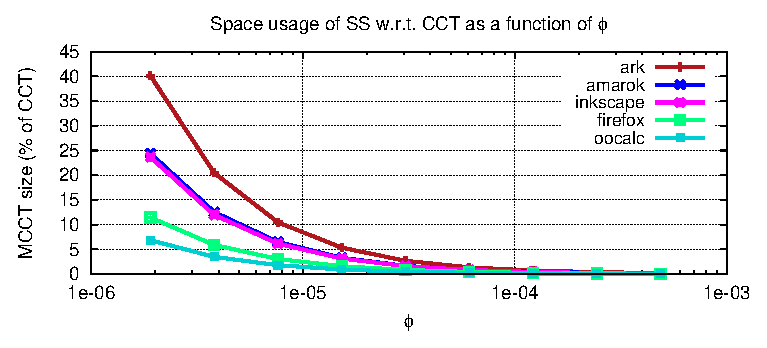
\includegraphics[width=0.75\textwidth]{figures/hcct-space-by-phi/hcct-space-by-phi.eps}
\caption{\protect\label{fig:hcct-space-by-phi} Space usage as a function of the hotness threshold $\phi$..
}
\end{center}
\end{figure}
\fi

\ifdefined\noauthorea
\begin{figure}[!ht]
\begin{center}
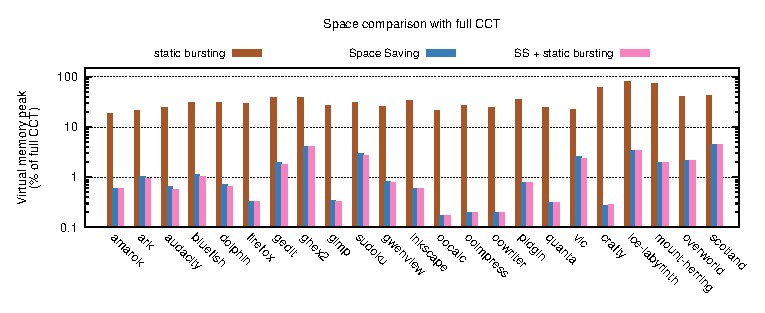
\includegraphics[width=\textwidth]{figures/hcct-space/hcct-space.eps}
\caption{\protect\label{fig:hcct-space} Space analysis of static bursting (left), SS (center), and SS combined with static bursting (right) with sampling interval 2 msec and burst length 0.2 msec.

%Space analysis on several benchmarks of static bursting~\cite{Zhuang06} (left), SS (center), and SS combined with static bursting (right) with sampling interval 2 msec and burst length 0.2 msec.

}
\end{center}
\end{figure}
\fi

As a second experiment, we study the actual memory footprint of our profilers considering both SS and the combination of SS with static bursting. \myfigure\ref{fig:hcct-space} plots the peak memory usage of our profilers as a percentage of the full CCT. We recall that during the computation we store the minimal subtree MCCT of the CCT spanning all monitored contexts. This subtree is eventually pruned to obtain the $(\phi,\varepsilon)$-HCCT (\mysection\ref{ss:hcct-approach,ss:hcct-algorithms}). The peak memory usage is proportional to the number of MCCT nodes, which is typically much larger than the actual number of hot contexts obtained after pruning.

Quite surprisingly, static bursting also improves space usage. This depends on the fact that sampling reduces the variance of calling context frequencies: MCCT cold nodes that have a hot descendant are more likely to become hot when sampling is active, and monitoring these nodes reduces the total MCCT size. The histogram also shows that static bursting alone (i.e., without streaming) is not sufficient to substantially reduce space: in addition to hot contexts, a large fraction of cold contexts is also sampled and included in the CCT. We also observed that the larger the applications, the larger the space reduction of our approach over bursting alone.

Since the average node degree is a small constant, cold HCCT nodes are typically a fraction of the total number of nodes, as shown in \myfigure\ref{fig:hcct-false-positives} for $\phi=10^{-4}$\ifauthorea{}{ (page \pageref{fig:hcct-false-positives})}. In our experiments we observed that this fraction strongly depends on the  hotness threshold $\phi$, and in particular decreases with $\phi$: cold nodes that have a hot descendant are indeed more likely to become hot when $\phi$ is smaller.

\subsection{Time Overhead}

We now discuss the time overhead of our approach, both alone and in combination with static bursting. We compare to native execution, to the widely-used call-graph profiler \gprof~\cite{Graham82}, and to the canonical CCT construction. To assess the instrumentation overhead, we also compare to {\em empty} instrumentation (i.e., when no analysis is performed).

\ifdefined\noauthorea
\begin{figure}[!ht]
\begin{center}
\begin{tabular}{cc}
\hspace{-6mm}
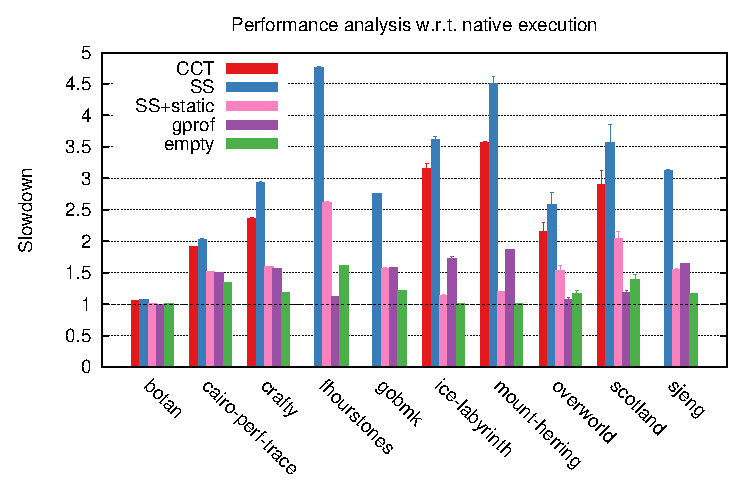
\includegraphics[width=0.49\textwidth]{figures/hcct-slowdown/hcct-slowdown-native.eps} &
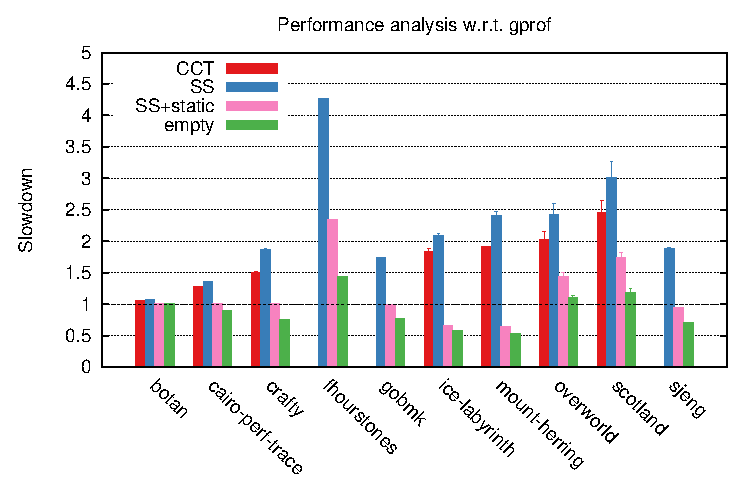
\includegraphics[width=0.49\textwidth]{figures/hcct-slowdown/hcct-slowdown-gprof.eps}\\
(a) & (b)
\end{tabular}
\caption{\protect\label{fig:hcct-slowdown} Runtime analysis for CCT and $(\phi,\varepsilon)$-HCCT construction compared to (a) native executions and (b) executions under \gprof. The {\em empty} bars measure the cost of instrumenting function calls and returns. SS with stating bursting has been executed with sampling interval 20 msec and burst length 2 msec.
}
\end{center}
\end{figure}
\fi

\myfigure\ref{fig:hcct-slowdown}(a) shows the overheads of the different profilers normalized against the performance of a native execution. The average slowdown for the CCT construction is $2.45\times$, with a peak of $3.56\times$ for {\tt mount-herring}. Note that data for benchmarks {\tt fhourstones}, {\tt gobmk} and {\tt sjeng} are not reported for the CCT profiler as it ran out of memory. We observe that the construction of the $(\phi,\varepsilon)$-HCCT incurs an average slowdown of $2.9\times$ ($3.09\times$ considering also OOM benchmarks) and is $16.28\%$ slower than the CCT profiler, with a peak of $26.08\%$ for {\tt mount-herring}. Given the previously discussed memory usage reduction, this represents an interesting space-time trade-off.

The integration with static bursting reduces the average overhead of our approach to $1.58\times$ for the whole set of benchmarks, which is not far from the $1.21\times$ slowdown introduced by the {\tt gcc} instrumentation itself. We observe a peak of $2.62\times$ on the benchmark {\tt fhourstones}: we believe this is due to the particular structure of its source code, which contains very frequently invoked tiny functions that could be replaced with macros.

In \myfigure\ref{fig:hcct-slowdown}(b) we have normalized the runtime overheads against an execution under \gprof. The combination of our approach with static bursting is very effective, as it is on average $18\%$ ($5.16\%$ if we exclude {\tt fhourstones}) slower than \gprof. On 5 out of 10 benchmarks, the two tools achieve nearly-identical slowdowns. We observe $2.34\times$, $1.44\times$ and $1.74\times$ slowdowns on {\tt fhourstones}, {\tt overworld}, and {\tt scotland}, respectively. Notice that for all these benchmarks the cost of the instrumentation inserted by \gcc\ is already greater than the slowdown introduced by \gprof. On the other hand, we observe appreciable speedups on {\tt ice-labyrinth} and {\tt mount-herring}, for which SS combined with static bursting is $1.51\times$ and $1.55\times$ faster than \gprof, respectively.

\subsection{Accuracy}
% !TEX root = thesis.tex

%\section{{\em k-}iteration Path Profiling}
\section{Multi-iteration Path Profiling}
\label{ss:kblpp-eval}

In this section, we discuss and evaluate an implementation, which we call \kblpp, of our approach to multi-iteration path profiling in the Jikes Research Virtual Machine (RVM)~\cite{Alpern00}. Our code is publicly available in the Jikes RVM Research Archive\footnote{\url{http://sourceforge.net/p/jikesrvm/research-archive/41/}.} and has been endorsed by the OOPSLA 2013 Artifact Evaluation Committee. The goal of our experimental study is to assess the performance of our profiler compared to previous approaches and to study properties of path profiles that span multiple iterations for several representative benchmarks. The results indicate that our technique can profile paths that extend across many loop iterations in a time comparable with acyclic path profiling on a large variety of industrial-strength benchmarks.

\subsection{Implementation}
\label{ss:kblpp-implementation}

\paragraph*{Adaptive Compilation.}  Jikes RVM is a high-performance {\em meta-circular} virtual machine: unlike most other JVMs, it is written in Java. Jikes RVM does not include an interpreter: all bytecode must be first translated into native machine code. The unit of compilation is the method, and methods are compiled lazily by a fast non-optimizing compiler -- the so-called {\em baseline} compiler -- when they are first invoked by the program. As execution continues, the Adaptive Optimization System monitors program execution to detect program hot spots and selectively recompiles them with three increasing levels of optimization. This approach is typical of modern production JVMs, which rely on some variant of selective optimizing compilation to target the subset of the hottest program methods where they are expected to yield the most benefits.

Recompilation is performed by the {\em optimizing} compiler, that generates higher-quality code but at a significantly larger cost than the baseline compiler. Since Jikes RVM quickly recompiles frequently executed methods, we implemented \kblpp in the optimizing compiler only.

\paragraph*{Adding Instrumentation.} As discussed in \mysection\ref{ss:kblpp-approach}, the Ball-Larus tracing technique requires instrumenting CFG edges so that when an edge is traversed, the probe value is incremented by a quantity computed by the path numbering algorithm on the DAG obtained by transforming back edges in the CFG.

\kblpp\ adds instrumentation to hot methods in three passes:
\begin{enumerate}[itemsep=0pt]
 \item building the DAG representation;
 \item assigning values to edges;
 \item adding instrumentation to edges.
\end{enumerate}

\noindent \kblpp\ adopts the {\em smart path numbering} algorithm proposed by Bond and McKinley~\cite{Bond05b} to improve performance by placing instrumentation on cold edges. In particular, line 6 of the canonical Ball-Larus path numbering algorithm shown in \myalgorithm\ref{alg:kblpp-bl-numbering} \ifauthorea{}{(page \pageref{alg:kblpp-bl-numbering})} is modified such that outgoing edges are picked in decreasing order of execution frequency. For each basic block edges are sorted using existing edge profiling information collected by the baseline compiler: we can thus assign zero to the hottest hedge, so that \kblpp\ will not place any instrumentation on it.
%in this way we can assign zero to the hottest edge, thus allowing us to assign zero to the hottest edge so that \kblpp\ does not place any instrumentation on it.

During compilation, Jikes RVM introduces {\em yield points}, which are program points where the running thread determines whether it should yield to another thread. Since JVMs need to gain control of threads quickly, compilers insert yield points in method prologues, loop headers, and method epilogues. We modified the optimizing compiler to also store the path profiling probe on loop headers and method epilogues. Ending paths at loop headers rather than back edges causes a path that traverse a header to be split into two paths: this difference from canonical Ball-Larus path profiling is minor because it only affects the first path through a loop~\cite{Bond05}.

Note that optimizing compilers do not insert yield points in a method when either it does not contain branches (hence its profile is trivial) or it is marked as uninterruptible. The second case occurs in internal Jikes RVM methods only; the compiler occasionally inlines such a method into an application method, and this might result in a loss of information only when the execution reaches a loop header contained in the inlined method. However, according to \cite{Bond05}, this loss of information appears to be negligible.

\paragraph*{Path Profiling.} To make fair performance comparisons with state-of-the-art previous profilers, we built our code on top of the BLPP profiler developed by Bond~\cite{Bond05,PEP}, which provides an efficient implementation of the Ball-Larus acyclic-path profiling technique. The \ksf\ construction algorithm described in \mysection\ref{ss:kblp-algorithms} is implemented using a standard first-child, next-sibling representation for nodes. This representation is very space-efficient, as it requires only two pointers per node: one to its leftmost child and the other to its right nearest sibling. % - while experimental results show that the average degree of a node is usually low.

\ifdefined\noauthorea
\begin{figure}[!ht]
\begin{center}
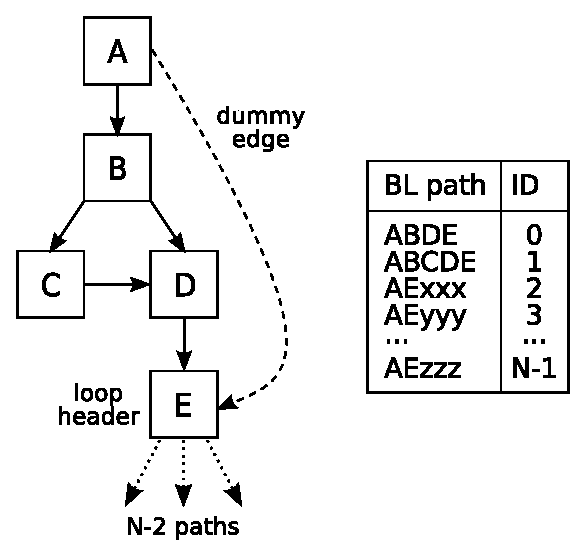
\includegraphics[width=0.4\textwidth]{figures/kblpp-example-fewer/kblpp-example-fewer.eps}
\caption{\protect\label{fig:kblpp-example-fewer} Routine with an initial branch before the first cycle.}
\end{center}
\end{figure}
\fi

\noindent Tree roots are stored and accessed through an efficient implementation\footnote{{\tt HashMapRVM} is a stripped-down implementation of the {\tt HashMap} data structure used by core parts of the Jikes RVM runtime and by Bond's BLPP path profiler.} of a hash map, using the pair represented by the Ball-Larus path ID and the unique identifier associated to the current routine (i.e., the compiled method ID) as key. Note that this map is typically smaller than a map required by a traditional BLPP profiler, since tree roots represent only a fraction of the distinct path IDs encountered during the execution. Consider, for instance, the example shown in \myfigure\ref{fig:kblpp-example-fewer}: this control flow graph has $N$ acylic paths after backedges have been removed. Since cyclic paths are truncated on loop headers, only path IDs $0$ and $1$ can appear after the special marker $*$ in the stream, thus leading to the creation of an entry in the hash map. Additional entries might be created when a new tree is added to the \ksf\ (line 10 of the streaming algorithm shown in \myalgorithm\ref{alg:kblpp-ksf-algorithm}\ifauthorea{}{ on page \pageref{alg:kblpp-ksf-algorithm}}); however, experimental results show that the number of tree roots is usually small, while $N$ increases with the complexity (i.e., number of branches and loops) of the routine.

\subsection{Experimental Setup}

In this section we illustrate the details of our experimental methodology, focusing on benchmarks, performance and topological metrics, and compared profiling techniques.

\subsubsection*{Benchmarks}

We evaluated \kblpp\ against a variety of prominent benchmarks drawn from three suites. The \dacapo\ suite~\cite{Blackburn06} consists of a set of open source, real-world applications with non-trivial memory loads. We use the superset of all benchmarks from \dacapo\ releases 2006-10-MR2 and 9.12 that can run successfully in Jikes RVM, using the largest available workload for each benchmark. In particular, {\tt avrora}, {\tt jython}, {\tt luindex}, {\tt sunflow}, and {\tt xalan} are taken from the 9.12 release, while {\tt chart}, {\tt eclipse}, and {\tt hsqldb} are from the 2006-10-MR2 release.

The \specjvm\ suite~\cite{SpecJVM2008} focuses on the performance of the hardware processor and memory subsystem when executing common general purpose application computations. Benchmarks from the suite that can run successfully\footnote{Due to limitations of the GNU classpath, only a small number of them are supported.} on Jikes RVM include: {\tt compiler.compiler}, {\tt compress}, {\tt mpegaudio}, and {\tt scimark.\{montecarlo, sor.large, sparse.large\}}.

Finally, we chose two memory-intensive benchmarks ({\tt heapsort} and {\tt md}) from the \javagrande\ $2.0$ suite~\cite{Bull99} to further evaluate the performance of \kblpp.

\subsubsection*{Metrics}
We considered a variety of metrics, including wall-clock time, number of operations per second performed by the profiled program, number of hash table operations, data structure size (e.g., number of hash table items for \blpp\ and number of \ksf\ nodes for \kblpp), and statistics such as average node degree of the \ksf\ and the \kipf\ and average depth of \kipf\ leaves. To interpret our results, we also ``profiled our profiler'' by collecting hardware performance counters with {\tt perf}~\cite{perf}, including L1 and L2 cache miss rate, branch mispredictions, and cycles per instruction (CPI).

\subsubsection*{Compared Codes}
In our experiments, we analyzed the native (uninstrumented) version of each benchmark and its instrumented counterparts, comparing \kblpp\ for different values of $k$ (2, 3, 4, 6, 8, 11, 16) with the \blpp\ profiler developed by Bond~\cite{PEP} for Ball-Larus acyclic-path profiling. We upgraded the original tool by Bond to take advantage of native threading support introduced in later Jikes RVM releases; the code is structured as in \myfigure\ref{fig:kblpp-approach}\ifauthorea{}{ (page \pageref{fig:kblpp-approach})}, except that it does not produce any intermediate stream, but it directly performs {\tt count[r]++}.

\subsubsection*{Platform}
In our experiments we used a 2.53GHz Intel Core2 Duo T9400 with 128KB of L1 data cache, 6MB of L2 cache, and 4 GB of main memory DDR3 1066, running Ubuntu 12.10, Linux Kernel 3.5.0, 32 bit. We ran all of the benchmarks on Jikes RVM 3.1.3 (default {\tt production} build) using a single core and a maximum heap size equal to half of the amount of physical memory. For each benchmark/profiler combination, we performed 10 trials, each preceded by a warm-up execution, and computed the arithmetic mean. We collected performance measurements with negligible background activity. We report confidence intervals stated at 95\% confidence level.

\subsection{Time Overhead}
\label{ss:eval-kblpp-time}

In \myfigure\ref{fig:kblpp-slowdown} we report for each benchmark the profiling overhead of \kblpp\ relative to \blpp. The chart shows that for 12 out of 16 benchmarks the overhead decreases for increasing values of $k$, providing up to almost 45\% improvements over \blpp. This is explained by the fact that hash table accesses are performed by {\tt process\_bl\_path\_id} every $k-1$ items read from the input stream between two consecutive routine entry events (lines 8 and 10 in \myalgorithm\ref{alg:kblpp-ksf-algorithm}\ifauthorea{)}{on page \pageref{alg:kblpp-ksf-algorithm})}. As a consequence, the number of hash table operations for each routine call is $O(1+N/(k-1))$, where $N$ is the total length of the path taken during the invocation.

\ifdefined\noauthorea
\begin{figure}[!ht]
\begin{center}
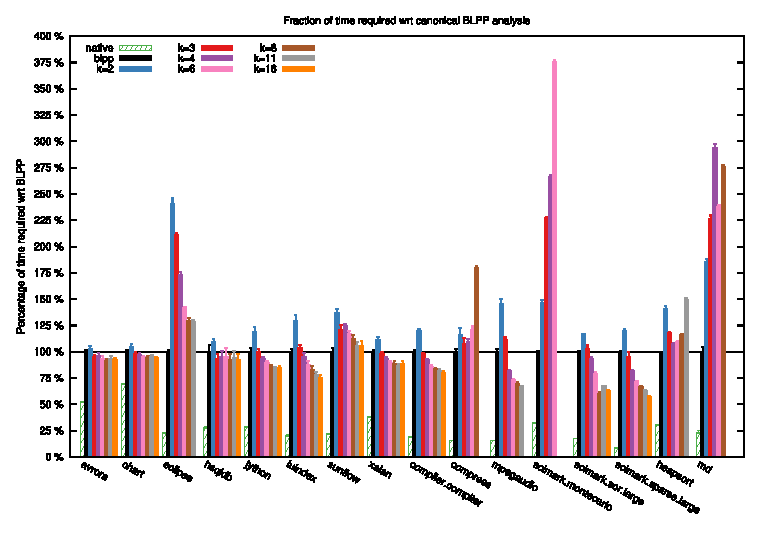
\includegraphics[width=\textwidth]{figures/kblpp-slowdown/kblpp-slowdown.eps}
\caption{\protect\label{fig:kblpp-slowdown} Performance of \kblpp\ relative to \blpp.
}
\end{center}
\end{figure}
\fi

In \myfigure\ref{fig:kblpp-hash} we report the measured number of hash table accesses for our experiments, which decreases as predicted on all benchmarks with intense loop iteration activity. Notice that not only does \kblpp\ perform fewer hash table operations, but since only a subset of BL path IDs are inserted, the table is also smaller, thus yielding further performance improvements. For codes such as {\tt avrora} and {\tt hsqldb}, which perform on average a small number of iterations, increasing $k$ beyond this number does not yield any benefit.

\ifdefined\noauthorea
\begin{figure}[!ht]
\begin{center}
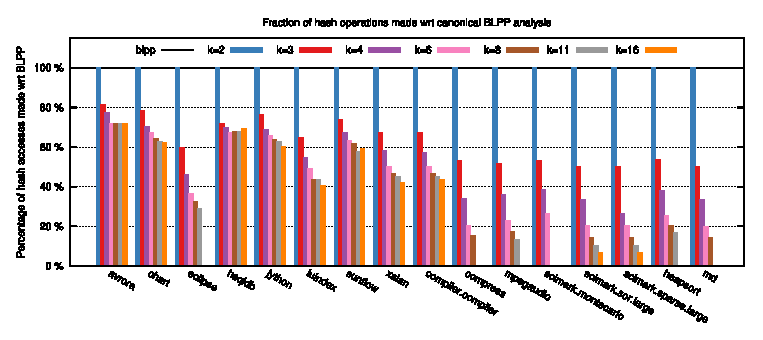
\includegraphics[width=\textwidth]{figures/kblpp-hash/kblpp-hash.eps}
\caption{\protect\label{fig:kblpp-hash} Number of hash table operations performed by \kblpp\ relative to \blpp.
}
\end{center}
\end{figure}
\fi

On {\tt eclipse}, \kblpp\ gets faster as $k$ increases, but differently from all other benchmarks in this class, it remains slower than \blpp\ by at least 25\%. The reason is that, due to structural properties of the benchmark, the average number of node scans at lines 13 and 21 of {\tt process\_bl\_path\_id} is rather high (58.8 for $k=2$ down to 10.3 for $k=16$). In contrast, the average degree of internal nodes of the \ksf\ is small (2.6 for $k=2$ decreasing to 1.3 for $k=16$), hence there is intense activity on nodes with a high number of siblings. No other benchmark exhibited this extreme behavior. We expect that a more efficient implementation of {\tt process\_bl\_path\_id}, e.g., by adaptively moving hot children to the front of the list, could reduce the scanning overhead for this kind of worst-case benchmarks as well.

\noindent Benchmarks {\tt compress}, {\tt scimark.montecarlo}, {\tt heapsort}, and {\tt md} made an exception to the general trend we observed, with performance overhead increasing, rather than decreasing, with $k$. To explain this behavior, we collected and analyzed several hardware performance counters and noticed that on these benchmarks our \kblpp\ implementation suffers from increased CPI for higher values of $k$.

\ifdefined\noauthorea
\begin{figure}[!ht]
\begin{center}
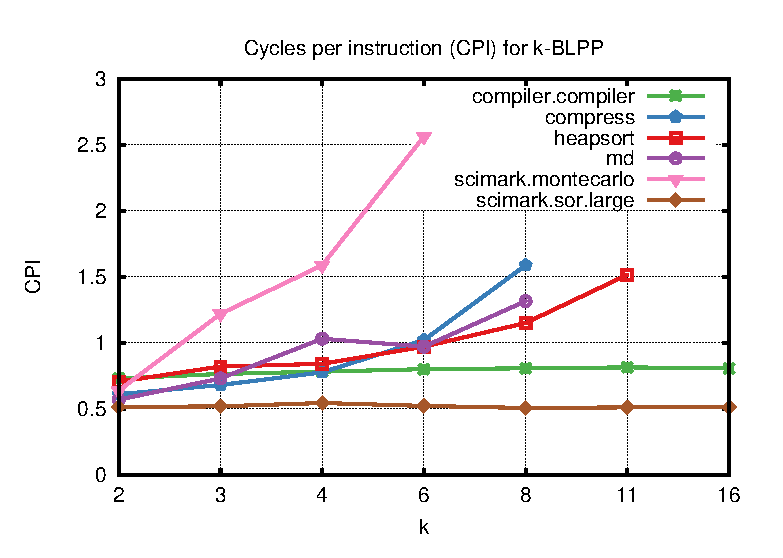
\includegraphics[width=0.49\textwidth]{figures/kblpp-cpi/kblpp-cpi.eps}
\caption{\protect\label{fig:kblpp-cpi} Hardware performance counters for \kblpp: cycles per instruction (CPI).
}
\end{center}
\end{figure}
\fi

\vspace{2em}
\noindent\myfigure\ref{fig:kblpp-cpi} shows this phenomenon, comparing the four outliers with other benchmarks in our suite. By analyzing L1 and L2 cache miss rates, reported in \myfigure\ref{fig:kblpp-cache} (a) and \myfigure\ref{fig:kblpp-cache} (b), we noticed that performance degrades due to poor memory access locality. We believe this to be an issue of our current implementation of \kblpp, in which we did not make any effort aimed at improving cache efficiency in accessing the \ksf, rather than a limitation of the general approach we propose. Indeed, as nodes may be unpredictably scattered in memory due to the linked structure of the forest, pathological situations may arise where node scanning incurs several cache misses.

\ifdefined\noauthorea
\begin{figure}[!ht]
\begin{center}
\begin{tabular}{cc}
\hspace{-6mm}
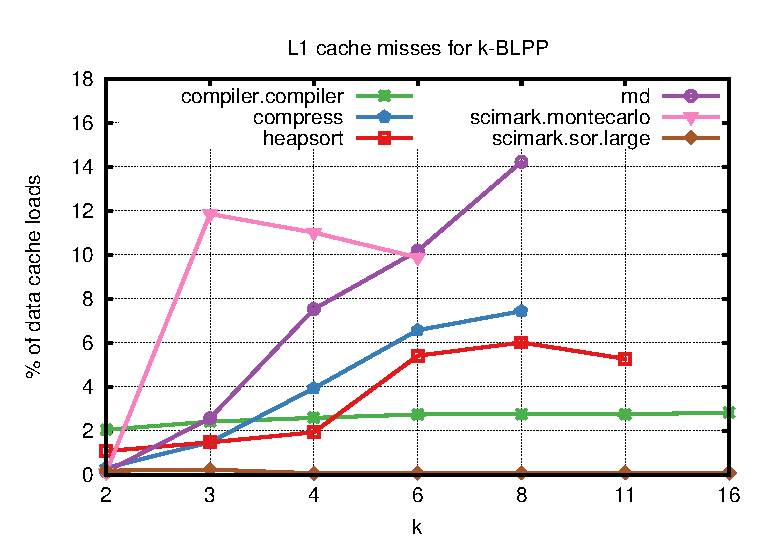
\includegraphics[width=0.49\textwidth]{figures/kblpp-cache/kblpp-cache-L1.eps} &
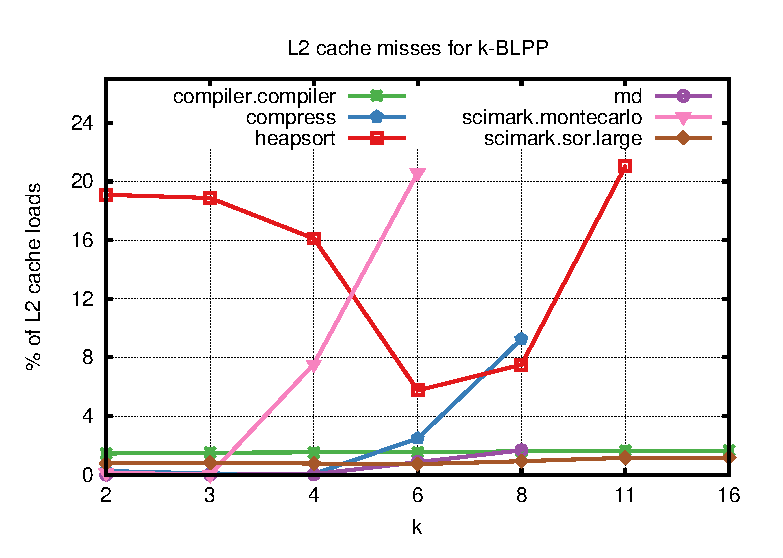
\includegraphics[width=0.49\textwidth]{figures/kblpp-cache/kblpp-cache-L2.eps}\\
(a) & (b)
\end{tabular}
\caption{\protect\label{fig:kblpp-cache} Hardware performance counters for \kblpp: (a) L1 and (b) L2 cache miss rates.}
\end{center}
\end{figure}
\fi

%\noindent Notice that since we never delete either entries from the hash table or nodes from the \ksf, our implementation does not place any additional burden on the garbage collector. The profiler causes memory release operations only when a thread terminates, dumping all of its data structures at once.

\noindent Notice that since we never delete either entries from the hash table or nodes from the \ksf, the only load we place on the garbage collector comes from allocating new nodes when needed. In fact, the profiler causes memory release operations only when a thread terminates, dumping all of its data structures at once.

\subsection{Memory Usage and Structural Properties}
\myfigure\ref{fig:kblpp-space} compares the space requirements of \blpp\ and \kblpp\ for different values of $k$. The chart reports the total number of items stored in the hash table by \blpp\ and the number of nodes in the \ksf.

\ifdefined\noauthorea
\begin{figure}[!ht]
\begin{center}
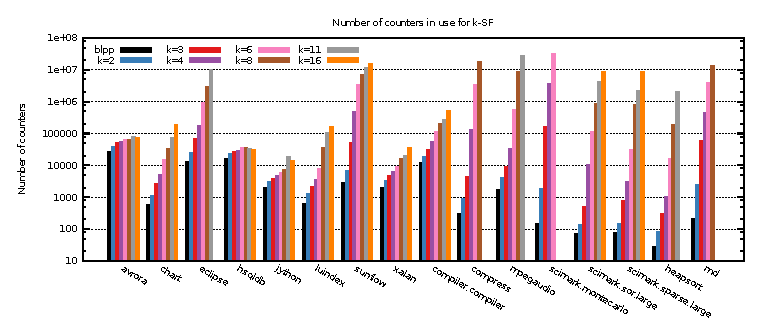
\includegraphics[width=\textwidth]{figures/kblpp-space/kblpp-space.eps}
\caption{\protect\label{fig:kblpp-space} Space requirements: number of hash table entries in \blpp\ and number of nodes in the \ksf.

}
\end{center}
\end{figure}
\fi

\vspace{-1em}

\ifdefined\noauthorea
\begin{figure}[!ht]
\begin{center}
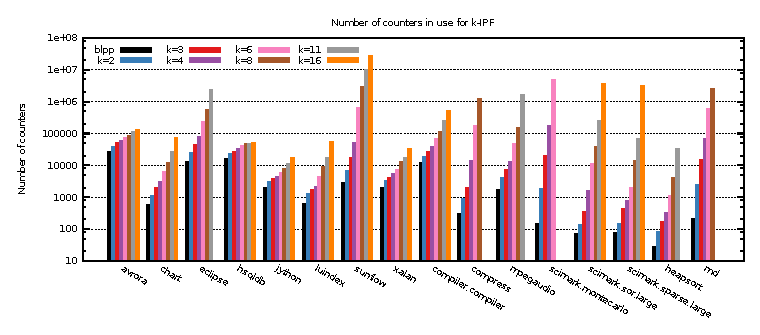
\includegraphics[width=\textwidth]{figures/kblpp-space-kipf/kblpp-space-kipf.eps}
\caption{\protect\label{fig:kblpp-space-kipf} Number of paths profiled by \blpp\ and \kblpp.

}
\end{center}
\end{figure}
\fi

\noindent Since both \blpp\ and \kblpp\ exhaustively encode exact counters for all distinct taken paths of bounded length, space depends on intrinsic structural properties of the benchmark. Programs with intense loop iteration activity are characterized by substantially higher space requirements by \kblpp, which collects profiles containing up to several millions of paths. Notice that on some benchmarks we ran out of memory for large values of $k$, hence some bars in the charts we report in this section are missing. In \myfigure\ref{fig:kblpp-space-kipf} we report the number of nodes in the \kipf, which corresponds to the number of paths profiled by \kblpp. Notice that since a path may be represented more than once in the \ksf, the \kipf\ represents a more compact version of the \ksf.

\noindent As a final experiment, we measured structural properties of the \kipf\ such as average degree of internal nodes (\myfigure\ref{fig:kblpp-kipf-degree}) and the average leaf depth (\myfigure\ref{fig:kblpp-kipf-leaves}). Our tests reveal that the average node degree generally decreases with $k$, showing that similar patterns tend to appear frequently across different iterations. Some benchmarks, however, such as {\tt sunflow} and {\tt heapsort} exhibit a larger variety of path ramifications, witnessed by increasing node degrees at deeper levels of the \kipf. The average leaf depth allows us to characterize the loop iteration activity of different benchmarks. Notice that for some benchmarks, such as {\tt avrora} and {\tt hsqldb}, most cycles consist of a small number of iterations: hence, by increasing $k$ beyond this number, \kblpp\ does not collect any additional useful information.

\ifdefined\noauthorea
\begin{figure}[!ht]
\begin{center}
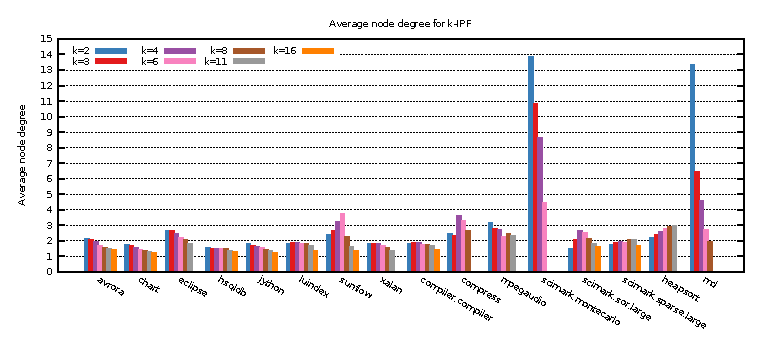
\includegraphics[width=\textwidth]{figures/kblpp-kipf-degree/kblpp-kipf-degree.eps}
\caption{\protect\label{fig:kblpp-kipf-degree} Average degree of \kipf\ internal nodes.

}
\end{center}
\end{figure}
\fi

\vspace{-1em}

\ifdefined\noauthorea
\begin{figure}[!ht]
\begin{center}
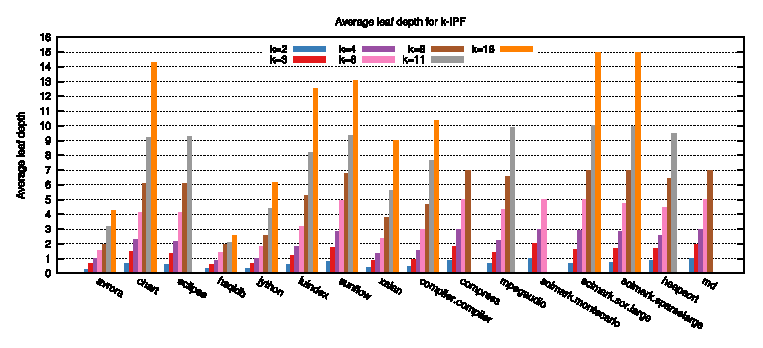
\includegraphics[width=\textwidth]{figures/kblpp-kipf-leaves/kblpp-kipf-leaves.eps}
\caption{\protect\label{fig:kblpp-kipf-leaves} Average depth of \kipf\ leaves.

}
\end{center}
\end{figure}
\fi

\subsection{Discussion}
Compared to previous approaches that enumerate $k$-iteration paths explicitly using numerical identifiers (\mysection\ref{ss:kblpp-related}), our prefix forest-based solution resorts to the original Ball-Larus encoding algorithm and maintains an intermediate data structure, the \ksf, that can be updated in constant time regardless of the value of $k$. Our technique can be faster than the original Ball-Larus algorithm on large programs, as it performs fewer operations on possibly smaller hash tables; for the same reason, its run-time overhead typically decreases for increasing values of $k$. We believe that our implementation is amenable to interesting enhancements, for instance by devising pruning heuristics in order to scale to larger values of $k$, or by having a separate thread construct the \ksf\ from the stream of BL path IDs emitted by an instrumented program's thread.

% !TEX root = thesis.tex

\section{OSR in LLVM}
\label{se:eval-osrkit}

In this section we present an experimental study of \osrkit. In particular, we aim at addressing the following questions:

\begin{description}[labelindent=1em ,labelsep*=1em,leftmargin=3.5em,itemsep=3pt,parsep=3pt]
\item[Q1] How much does a never-firing OSR point impact code quality? What kind of slowdown should we expect?
\item[Q2] What is the run-time overhead of an OSR transition, for instance to a clone of the running function?
\item[Q3] What is the overhead of \osrkit\ for inserting OSR points and creating a stub or a continuation function?
\end{description}

\noindent Experimental results suggest that inserting an OSR point is unlikely to degrade the quality of generated code, and that the time spent in IR manipulation is likely to be dominated by compilation costs. For an optimizer, the choice whether to insert an OSR point into a function merely depends on the trade-off between the expected benefits in terms of execution time and the overhead from generating the new code version: compared to this task, the cost of OSR-related operations is negligible.

\subsection{Experimental Setup}

\subsubsection*{Benchmarks}
We address questions Q1-Q3 by analyzing the performance of \osrkit\ on a selection of the \shootout\ benchmarks, also known as the Computer Language Benchmarks Game~\cite{shootout}, running in \tinyvm. In particular, we focus on single-threaded benchmarks that do not rely on external libraries to perform their core computations. Benchmarks and their description are reported in \mytable\ref{tab:osr-shootout}; four of them ({\tt b-trees}, {\tt mbrot}, {\tt n-body} and {\tt sp-norm}) are evaluated against two workloads of different size.

We generate the IR modules for our experiments with \clang\ starting from the C version of the \shootout\ suite. To cover scenarios where OSR machinery is inserted in programs with different optimization levels, we consider two versions: 1) {\em unoptimized}, where the only LLVM optimization we perform is \memtoreg\ to promote stack references to registers and construct the SSA form; 2) {\em optimized}, where we apply {\tt opt} {\tt -O1} to the unoptimized version.

\begin{table}[!hb]
\begin{center}
\begin{small}
    \begin{tabular}{ |c|c| }
        \hline
        Benchmark & Description \\
        \hline
        \hline
        b-trees & Adaptation of a GC bench for binary trees \\
        \hline
        fannkuch & Fannkuch benchmark on permutations \\
        \hline
        fasta & Generation of DNA sequences \\
        \hline
        fasta-redux & Generation of DNA sequences (with lookup table) \\
        \hline
        mbrot & Mandelbrot set generation \\
        \hline
        n-body & N-body simulation of Jovian planets \\
        \hline
        rev-comp & Reverse-complement of DNA sequences \\
        \hline
        sp-norm & Eigenvalue calculation with power method \\
        \hline
    \end{tabular}
\end{small}
\end{center}
\caption{\label{tab:osr-shootout} Description of the \shootout\ benchmarks.}
\end{table}

\subsubsection*{Environment}
\tinyvm\ supports interactive invocations of functions and it can compile LLVM IR either generated at run time or loaded from disk. The main design goal behind \tinyvm\ is the creation of an interactive environment for IR manipulation and JIT-compilation of functions: for instance, it allows the user to insert OSR points in loaded functions, run optimization passes on them or display their CFGs, repeatedly invoke a function for a specified amount of times and so on.

\tinyvm\ supports dynamic library loading and linking, and comes with a helper component for MCJIT that simplifies tasks such as handling multiple IR modules, symbol resolution in the presence of multiple versions of a function, and tracking native code and other machine-level generated object such as Stackmaps (\mysection\ref{ss:osrkit-implementation}). \tinyvm\ is thus an ideal playground to exercise our OSR technique.

\subsubsection*{Platform}
We performed our experiments on an octa-core 2.3Ghz Intel Xeon E5-4610 v2 with 256+256KB of L1 cache, 2MB of L2 cache, 16MB of shared L3 cache, and 128 GB of DDR3 main memory, running Debian Wheezy 7, Linux kernel 3.2.0, LLVM 3.6.2 (Release build, compiled using gcc 4.7.2), 64 bit. For each benchmark we analyze CPU time performing 10 trials preceded by an initial warm-up iteration; reported confidence intervals are stated at 95\% confidence level.

\subsection{Impact on Code Quality}

In order to measure how much a never-firing OSR point might impact code quality (Q1), we analyzed the source-code structure of each benchmark and profiled its run-time behavior to identify performance-critical sections for OSR point insertion. The distinction between open and resolved OSR points is nearly irrelevant in this context: we choose to focus on open OSR points, passing {\tt null} as the {\tt val} argument for the stub (see \mysection\ref{ss:osrkit-implementation}).

For iterative benchmarks, we insert an OSR point in the body of their hottest loops. We classify a loop as hottest when its body is executed for a very high cumulative number of iterations (e.g., from millions up to billions) and it either calls the method with the highest {\em self} time in the program, or it performs the most computational-intensive operations for the program in its own body.

\ifdefined\noauthorea
\begin{figure}[t]
\begin{center}
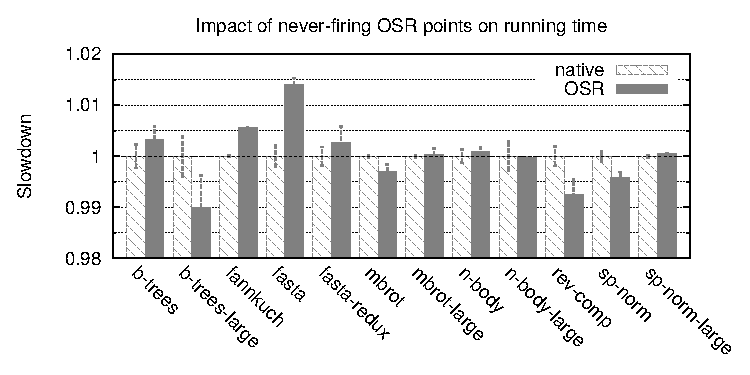
\includegraphics[width=0.65\textwidth]{figures/osr-code-quality-base/osr-code-quality-base.eps}
\caption{\protect\label{fig:osr-code-quality-base} Q1: Impact on running time of never-firing OSR points inserted inside hot code portions (unoptimized code).


}
\end{center}
\end{figure}
\fi

\ifdefined\noauthorea
\begin{figure}[t]
\begin{center}
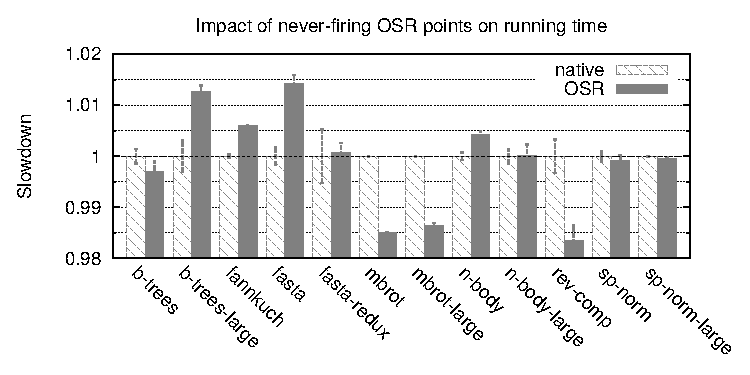
\includegraphics[width=0.65\textwidth]{figures/osr-code-quality-O1/osr-code-quality-O1.eps}
\caption{\protect\label{fig:osr-code-quality-O1} Q1: Impact on running time of never-firing OSR points inserted inside hot code portions (optimized code).



}
\end{center}
\end{figure}
\fi

These loops are natural candidates for OSR point insertion: for instance, Jikes RVM inserts yield points on backward branches to trigger operations such as method recompilation through OSR and thread preemption for garbage collection. In the \shootout\ benchmarks, the number of such loops is typically 1 (2 for {\tt spectral-norm}).

For recursive benchmarks, we insert an OSR point in the body of the method that accounts for the largest {\em self} execution time in the program. Such an OSR point might be useful to trigger recompilation of the code at a higher degree of optimization, enabling for instance multiple levels of inlining for non-tail-recursive functions. The only analyzed benchmark showing a recursive pattern is {\tt b-trees}.

Results for the unoptimized and optimized versions of the benchmarks are reported in \myfigure\ref{fig:osr-code-quality-base} and \myfigure\ref{fig:osr-code-quality-O1}, respectively. For both scenarios we observe that the overhead is very small, i.e., less than $1\%$ for most benchmarks and less than $2\%$ in the worst case. For some benchmarks, code might run slightly faster after OSR point insertion due to instruction cache effects.
%We analyzed the code produced by the x86-64 back-end: the OSR machinery is lowered into three native instructions that load a counter in a register, compare it against a constant value and jump to the OSR block accordingly.
The number of times the OSR condition is checked for each benchmark is
%the same as in the experiments
reported in \mytable\ref{tab:osr-sameFun}.

\subsection{Overhead of OSR Transitions}

\mytable\ref{tab:osr-sameFun} reports estimates of the average cost of performing an OSR transition to a clone of the running function (Q2). For each benchmark we compute the time difference between the scenarios in which an always-firing and a never-firing resolved OSR point is inserted in the code, respectively; we then normalize this difference against the number of fired OSR transitions.

\begin{table}[ht]
\begin{center}
\begin{small}
    \begin{tabular}{ |c|C{1.33cm}|C{1.00cm}|C{1.15cm}|C{1.00cm}|C{1.15cm}| }
        \cline{3-6}
        \multicolumn{2}{c|}{} & \multicolumn{2}{c|}{{\em Unoptimized code}} & \multicolumn{2}{c|}{{\em Optimized code}} \\
        \hline
        Benchmark & Fired OSRs (M) & Live values & Avg time (ns) & Live values & Avg time (ns) \\
        \hline
        \hline
        b-trees & 605 & 2 & 1.731 & 3 & 0.974 \\
        \hline
        b-trees-large & 2\,690 & 2 & 1.749 & 3 & 1.423 \\
        \hline
        fannkuch & 399 & 0 & 1.793 & 0 & 0.621 \\
        \hline
        fasta & 400 & 2 & 2.335 & 2 & 2.699 \\
        \hline
        fasta-redux & 400 & 4 & 2.306 & 4 & 2.269 \\
        \hline
        mbrot & 256 & 15 & 5.016 & 15 & 3.628 \\
        \hline
        mbrot-large & 1\,024 & 15 & 5.268 & 15 & 4.637 \\
        \hline
        n-body & 50 & 3 & 2.952 & 3 & 6.929 \\
        \hline
        n-body-large & 500 & 3 & 2.953 & 3 & 6.953 \\
        \hline
        rev-comp & 6 & 8 & -10.158 & 8 & 8.267 \\
        \hline
        sp-norm & 1\,210 & 2 & 0.772 & 2 & -0.030 \\
        \hline
        sp-norm-large & 19\,360 & 2 & 0.778 & 2 & -0.003 \\
        \hline
    \end{tabular}
\end{small}
\end{center}
\caption{\label{tab:osr-sameFun}Cost of OSR transitions to the same function. For each benchmark we report the number of fired OSR transitions (rounded to millions), the number of live values passed at the OSR point, and the average time for a transition.
}
\end{table}

\noindent Hot code portions for OSR point insertion have been identified as in the Q1 experiments for code quality. Depending on the characteristics of the hot loop, we either transform its body into a separate function and instrument its entrypoint, or, when the loop calls a method with a high self time, we insert an OSR point at the beginning of that method.

Normalized differences reported in the table represent a reasonable estimate of the average cost of firing an OSR transition, which consists in moving live values to stack locations or registers to match the calling convention and then invoking the OSR continuation function.
%, which in other words is the cost of performing a function call passing the live variables as arguments.
Reported numbers are in the order of nanoseconds, and might be negative due to instruction cache effects. We remark that for this experiment slicing the loop body is preferable to inserting an OSR point in it, as the continuation function should fire an OSR itself at the very next loop iteration and so on, possibly leading to an undesired stack growth.

\subsection{OSR Machinery Generation}

We now discuss the overhead of the \osrkit\ library for inserting OSR machinery in the IR of a function (Q3). \mytable\ref{tab:osr-instrTime} reports for each benchmark the number of IR instructions in the instrumented function and the time spent in the IR manipulation. Locations for OSR points are chosen as in the Q1 experiments, and the target function is a clone of the source function.

\begin{table}[ht]
\begin{center}
\begin{small}
    \begin{tabular}{ |c|c|c|c|c|c|c| }
        \cline{3-7}
        \multicolumn{2}{l|}{} & \multicolumn{2}{c|}{{\em Open OSR {\tiny$(\mu s)$}}} & \multicolumn{3}{c|}{{\em Resolved OSR  {\tiny$(\mu s)$}}} \\
        \cline{3-7}
        \multicolumn{2}{l|}{} & Insert & Gen. & Insert & \multicolumn{2}{|c|}{Generate \fosrto} \\
        \cline{1-2} \cline{6-7}
        Benchmark & \textbar IR\textbar & point & stub & point & Total & Avg/inst \\
        \hline
        \hline
        b-trees & 13 & 15.40 & 28.32 & 14.31 & 76.13 & 5.86 \\
        \hline
        fannkuch & 50 & 14.16 & 18.66 & 12.84 & 208.03 & 4.16 \\
        \hline
        fasta & 38 & 12.93 & 27.07 & 13.01 & 250.39 & 6.59 \\
        \hline
        fasta-redux & 55 & 13.79 & 23.44 & 9.32 & 258.36 & 4.70 \\
        \hline
        mbrot & 77 & 15.96 & 27.39 & 15.30 & 384.61 & 4.99 \\
        \hline
        n-body & 19 & 14.31 & 19.73 & 11.58 & 88.73 & 4.67  \\
        \hline
        rev-comp & 145 & 16.31 & 39.99 & 13.90 & 810.84 & 5.59 \\
        \hline
        sp-norm & 28 & 15.31 & 27.50 & 12.41 & 154.54 & 5.52 \\
        \hline
    \end{tabular}
\end{small}
\end{center}
\caption{\label{tab:osr-instrTime} Q3: OSR machinery insertion in optimized code. Time measurements are expressed in microseconds. Results for unoptimized code are very similar and thus not reported.}
\end{table}

\noindent For open OSR points, we report the time spent in inserting the OSR point in the function and in generating the stub; both operations do not depend on the size of the function. For resolved OSR points, we report the time spent in inserting the OSR point and in generating the \fosrto\ function.

Not surprisingly, constructing a continuation function takes longer than the other operations (i.e., up to 1 ms vs. 20-40 us), as it involves cloning and manipulating the body of the target function and thus depends on its size: \mytable\ref{tab:osr-instrTime} hence comes with an additional column in which time is normalized against the number of IR instructions in the target function.

%On our benchmarks, the overall cost of IR manipulation is in the order of hundreds of microseconds, and is thus very likely to be dominated by the cost of just-in-time compilation.

\subsection{Discussion}
Our results suggest that the LLVM MCJIT compiler is able to generate efficient native code for the OSR machinery inserted in performance-critical code sections. The overall cost of IR manipulation for inserting an OSR point insertion and generating a continuation function is in the order of hundreds of microseconds on our benchmarks, and will likely be dominated by the time spent in just-in-time compilation. We present an example of effective optimization enabled by \osrkit\ in \mysection\ref{se:CS-matlab}. 

%Hence, for a front-end the choice of whether to insert an OSR point for optimization essentially depends on the performance gains from recompilation.

%%%%%%%%%%%%%%%%%%%%%%%%%%%%%%%%%%%%%%%%%%%

%\section{On-Stack Replacement \`{a} la Carte}
%\section{OSR Mapping Generation}
\section{Building OSR Compensation Code}
\label{se:eval-OSR-alC}

In this section we evaluate our implementation in LLVM of the techniques for automatic OSR mapping construction described in \mysection\ref{se:osr-a-la-carte}. In particular, we investigate whether in the presence of a number of common compiler optimizations, the algorithm \buildcomp\ can offer an extensive ``menu'' of possible program points where OSR can safely occur, generating the possibly required compensation code in an automated fashion. Our experiments suggest that bidirectional OSR transitions can be supported almost everywhere in this setting.

\subsection{Experimental Setup}
\label{ss:bc-exp-setup}

\subsubsection*{Benchmarks and Environment}
We implemented our technique in \tinyvm, introducing a number of features to:
\begin{itemize}
 \item clone a function $f_{base}$ and apply a sequence of OSR-aware optimization passes, thus generating an optimized version $f_{opt}$;
 \item construct and compose OSR mappings for the applied transformations;
 \item for each feasible OSR point in $f_{base}$/$f_{opt}$, invoke \osrkit\ to materialize the compensation code $\chi$ produced by \reconstruct\ into a sequence of IR instructions for the OSR entry block of $f'_{opt}$/$f'_{base}$ (\mysection\ref{ss:osr-llvm-approach}).
\end{itemize}

\noindent We instrumented a number of standard LLVM optimization passes, including {\em aggressive dead code elimination} (ADCE), {\em constant propagation} (CP), {\em common subexpression elimination} (CSE), {\em loop-invariant code motion} (LICM), {\em sparse conditional constant propagation} (SCCP), and {\em code sinking} (Sink). We also instrumented a number of utility passes required by LICM, such as {\em natural loop canonicalization} (LC) and {\em LCSSA-form construction} (LCSSA). Optimizations performed by the back-end (e.g., instruction scheduling, register allocation, peephole optimizations) do not require instrumentation as we operate at the IR level.

We evaluated our technique on the \speccpu~\cite{Henning06} and the \phoronixpts~\cite{Phoronix} benchmarking suites, reporting data for a subset of their C/C++ benchmarks. We profiled each benchmark to identify the hottest method and generated the IR for it using \clang\ with no optimization enabled other than \memtoreg. Starting from this version of the IR, which we will refer to as {\em base}, we generated an {\em opt} version by applying all our instrumented LLVM optimizations.

The list of benchmarks and transformations that are effective on their hottest method is reported in \mytable\ref{tab:OSR-alC-bench-desc}. Numbers reported in \mytable\ref{tab:OSR-alC-bench-IR} for the IR manipulations performed by the transformations suggest that, while the {\em opt} version is typically shorter than its {\em base} counterpart, it might have a larger number of $\phi$-nodes (most of them are inserted during the LCSSA-form construction). We observed that SCCP was able to eliminate a large number of unreachable blocks for \mytt{ffmpeg}, while for the remaining benchmarks the majority of instruction deletions are performed by CSE, which replaces all of the uses of these instructions in the rest of the code with uses of equivalent available instructions.

\begin{table}[t]
\begin{center}
\begin{small}
\begin{tabular}{ |c|c|c|c|c|c|c|c|c|c| }
        \cline{3-10}
        \multicolumn{2}{l|}{} & \multicolumn{6}{c|}{Optimizations} & \multicolumn{2}{c|}{Utilities} \\
        \hline
        Suite & Benchmark & \em{ADCE} & \em{CP} & \em{CSE} & \em{SCCP} & \em{LICM} & \em{Sink} & \em{LC} & \em{LCSSA} \\
        \hline
        \hline
        \multirow{7}{*}{SPEC} & bzip2 & & & \checkmark & & \checkmark & \checkmark & & \checkmark \\
        \cline{2-10}
        & h264ref & \checkmark & & \checkmark & & \checkmark & \checkmark & \checkmark & \checkmark \\
        \cline{2-10}
        & hmmer & & & \checkmark & & \checkmark & \checkmark & & \checkmark \\
        \cline{2-10}
        & namd & \checkmark & \checkmark & \checkmark & \checkmark & \checkmark & \checkmark & & \checkmark \\
        \cline{2-10}
        & perlbench & \checkmark & & \checkmark & & \checkmark & \checkmark & \checkmark & \checkmark \\
        \cline{2-10}
        & sjeng & & & \checkmark & \checkmark & \checkmark & \checkmark & & \checkmark \\
        \cline{2-10}
        & soplex & & & \checkmark & \checkmark & \checkmark & \checkmark & & \\
        \hline
        \hline
        \multirow{5}{*}{PTS} & bullet & & \checkmark & \checkmark & & \checkmark & \checkmark & & \checkmark \\
        \cline{2-10}
        & dcraw & & & \checkmark & & \checkmark & \checkmark & \checkmark & \checkmark \\
        \cline{2-10}
        & ffmpeg & \checkmark & \checkmark & \checkmark & & \checkmark & \checkmark & \checkmark & \checkmark \\
        \cline{2-10}
        & fhourstones & & \checkmark & \checkmark & & \checkmark & & \checkmark & \checkmark \\
        \cline{2-10}
        & vp8 & & & \checkmark & & \checkmark & \checkmark & & \checkmark \\
        \hline
    \end{tabular}
\end{small}
%\end{adjustbox}
\end{center}
\caption{\label{tab:OSR-alC-bench-desc} Optimizations and utility passes effective on the hottest function of each benchmark. Optimization passes have been applied in the same order (left-to-right) as they appear in the table. Utility passes {\em LC} and {\em LCSSA} are pre-requisites of {\em LICM}.}
\end{table}

\begin{table}[!t]
\begin{center}
\begin{small}
\begin{tabularx}{0.9\textwidth}{|c|X|c|c|c|c|}
\cline{3-6}
\multicolumn{2}{l|}{} & \multicolumn{2}{c|}{base} & \multicolumn{2}{c|}{opt} \\
\hline
Benchmark & Function & $|\pi|$ & $|\phi|$ & $|\pi|$ & $|\phi|$ \\
\hline
\hline
bzip2 & mainSort & 657 & 32 & 596 & 44 \\
\hline
h264ref & SetupFastFullPelSearch & 671 & 28 & 576 & 36 \\
\hline
hmmer & P7Viterbi & 568 & 6 & 383 & 8 \\
\hline
namd & ComputeNonbondedUtil::calc\_pair\_ energy\_fullelect & 1737 & 159 & 1636 & 224 \\
\hline
perlbench & S\_regmatch & 5574 & 305 & 5001 & 355 \\
\hline
sjeng & std\_eval & 1940 & 93 & 1540 & 105 \\
\hline
soplex & SPxSteepPR::entered4X & 195 & 2 & 154 & 2 \\
\hline
bullet & btGjkPairDetector::getClosestPoints NonVirtual & 587 & 24 & 553 & 42 \\
\hline
dcraw & vng\_interpolate & 590 & 37 & 545 & 49 \\
\hline
ffmpeg & decode\_cabac\_residual\_internal & 618 & 34 & 462 & 40 \\
\hline
fhourstones & ab & 288 & 29 & 284 & 39 \\
\hline
vp8 & vp8\_full\_search\_sadx8 & 334 & 41 & 299 & 60 \\
\hline
\end{tabularx}

\vspace{6mm}

\begin{tabular}{|c|c|c|c|c|c|c|c|}
\hline
Benchmark & Added & Deleted & Hoisted & Sunk & $RAUW_I$ & $RAUW_C$ & $RAUW_A$ \\
\hline
\hline
bzip2 & 16 & 77 & 12 & 3 & 71 & 0 & 2 \\
\hline
h264ref & 9 & 105 & 4 & 21 & 102 & 0 & 0 \\
\hline
hmmer & 2 & 187 & 13 & 1 & 187 & 0 & 0 \\
\hline
namd & 68 & 169 & 36 & 73 & 145 & 17 & 0 \\
\hline
perlbench & 86 & 667 & 96 & 28 & 627 & 0 & 0 \\
\hline
sjeng & 13 & 413 & 20 & 34 & 412 & 1 & 0 \\
\hline
soplex & 0 & 41 & 2 & 4 & 41 & 0 & 0 \\
\hline
bullet & 26 & 60 & 37 & 3 & 51 & 1 & 0 \\
\hline
dcraw & 13 & 58 & 25 & 6 & 58 & 0 & 0 \\
\hline
ffmpeg & 11 & 168 & 9 & 17 & 52 & 51 & 0 \\
\hline
fhourstones & 14 & 20 & 3 & 0 & 14 & 2 & 0 \\
\hline
vp8 & 19 & 54 & 17 & 34 & 54 & 0 & 0 \\
\hline
\end{tabular}
\end{small}
%\end{adjustbox}
\end{center}
\caption{\label{tab:OSR-alC-bench-IR} Details on the IR manipulations on the hottest function of each benchmark. For each function we report the number of instructions $|\pi|$ ($|\phi|$ of which represent $\phi$-nodes) for both the {\em base} and the {\em opt} version. We then report the number of primitive actions for code manipulations tracked across the applied transformations. $RAUW_{\{A,C,I\}}$ is used to indicate \RAUWfull\ actions performed for some {$N$} having Argument, Constant, or Instruction type in LLVM.
}
\end{table}

\subsubsection*{Platform}
We performed our experiments on a machine equipped with an Intel Core i7-3632QM processor, running Ubuntu 14.10, LLVM 3.6.2 (Release build), 64 bit.

\subsection{OSR to Optimized Version}

\myfigure\ref{fig:osr-BC-BtoO} shows the fraction of program points that are feasible for an OSR from {\em base} to {\em opt} depending on the version of \reconstruct\ being used (\mysection\ref{ss:BC-implementation}).

Locations that can fire an OSR with no need of a compensation code (i.e., $\chi=\langle\rangle$) account for a limited fraction of all the potential OSR points (less than $10\%$ for most benchmarks). This suggests that optimizations can significantly modify a program's live state across program locations.

\begin{figure}[!t]
\begin{center}
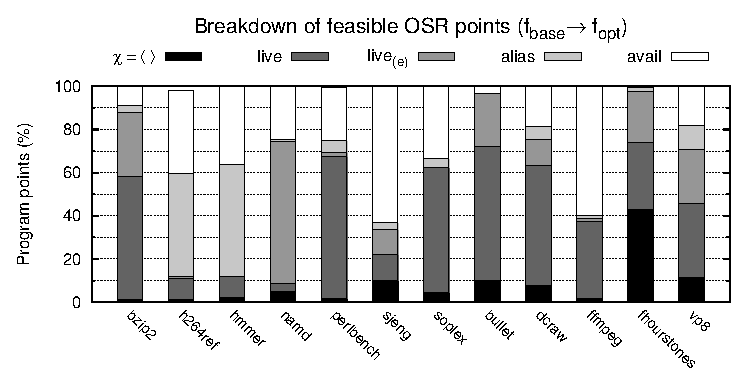
\includegraphics[width=0.8\textwidth]{figures/osr-BC-BtoO/osr-BC-BtoO.eps}
\caption{\protect\label{fig:osr-BC-BtoO} Fraction of program points that are OSR-feasible (from {\em base} to {\em opt}).

}
\end{center}
\end{figure}

We observe that the $live$ version of \reconstruct\ performs well on some benchmarks (e.g., \mytt{perlbench}, \mytt{bullet}, \mytt{dcraw}) and poorly on others (e.g., \mytt{h264ref}, \mytt{namd}). The enhancements introduced in the $live_{(e)}$ version are effective for some benchmarks (e.g., \mytt{namd}, \mytt{sjeng}), while aliasing information exploited in the $alias$ version increases the number of feasible OSR points for all benchmarks. For $9$ out of $12$ of them, it is possible in fact to build a compensation code using only live variables at the OSR source for more than $60\%$ of potential OSR points.

When in the $avail$ version \reconstruct\ is allowed to extend the liveness range of an ``available'' variable, the percentage of feasible OSR points grows to nearly $100\%$. We observed for \mytt{bullet} that a specific $\phi$-node needs to be reconstructed at nearly $20\%$ of feasible OSR points: this node takes as incoming values a number of $\phi$-nodes that in turn all yield the same value. While LLVM's built-in method for detecting trivially constant $\phi$-nodes does not cover this case, our recursive heuristic introduced in the $live_{(e)}$ version is able to identify the value and use it directly.

\begin{table}[!ht]
\begin{center}
\begin{small}
\begin{tabular}{ |c|c|c|c|c|c|c|c|c| }
\cline{2-9}
\multicolumn{1}{l|}{} & \multicolumn{2}{c|}{$|\chi|\leftarrow live_{(e)}$} & \multicolumn{2}{c|}{$|\chi|\leftarrow alias$} & \multicolumn{2}{c|}{$|\chi|\leftarrow avail$} & \multicolumn{2}{c|}{$|K_{avail}|$} \\
\hline
Benchmark & Avg & Max & Avg & Max & Avg & Max & Avg & Max \\
\hline
\hline
bzip2 & 4.29 & 14 & 4.3 & 14 & 4.73 & 13 & 3.6 & 8 \\
\hline
h264ref & 1.94 & 2 & 2.9 & 5 & 3.37 & 5 & 1.02 & 2 \\
\hline
hmmer & 3.3 & 5 & 16.11 & 23 & 16.63 & 24 & 4.02 & 7 \\
\hline
namd & 18.48 & 28 & 18.61 & 28 & 17.82 & 28 & 3.38 & 6 \\
\hline
perlbench & 46.29 & 57 & 46.12 & 57 & 45.82 & 57 & 1.24 & 12 \\
\hline
sjeng & 9.51 & 21 & 9.72 & 21 & 18.52 & 32 & 4.2 & 12 \\
\hline
soplex & 5.08 & 7 & 5.02 & 7 & 4.38 & 7 & 2.34 & 4 \\
\hline
bullet & 16.79 & 46 & 16.69 & 46 & 15.93 & 46 & 6.15 & 17 \\
\hline
dcraw & 7.72 & 15 & 7.6 & 15 & 7.32 & 15 & 1.97 & 7 \\
\hline
ffmpeg & 5.22 & 8 & 5.05 & 8 & 4.03 & 8 & 1.85 & 3 \\
\hline
fhourstones & 4.64 & 6 & 4.5 & 6 & 4.98 & 6 & 1.7 & 2 \\
\hline
vp8 & 9.6 & 16 & 10.51 & 16 & 10.13 & 17 & 2.35 & 6 \\
\hline
\hline
Avg & {\bf 11.07} & 18.75 & {\bf 12.26} & 20.50 & {\bf 12.81} & 21.50 & {\bf 2.82} & 7.17 \\
\hline
\end{tabular}
\end{small}
\end{center}
\caption{\label{tab:OSR-alC-prologue-BtoO} Average and peak size $|\chi|$ of the compensation code generated by the $live_{(e)}$, $alias$, and $avail$ versions of algorithm \reconstruct. $|K_{avail}|$ is the size of the set of variables that we should artificially keep alive in order to make program points represented by white bars in \myfigure\ref{fig:osr-BC-BtoO} feasible for an OSR from {\em base} to {\em opt}.}
\end{table}

In \mytable\ref{tab:OSR-alC-prologue-BtoO} we report the average and peak size of the compensation code $\chi$ generated by the $live_{(e)}$, $alias$, and $avail$ variants of \reconstruct\ across feasible OSR points. Figures for $live$ are not reported as they would not add much to the discussion. Note also that average values have been calculated for different sets of program points, although the set of a version includes the set of the previous version.

The assignment step of \reconstruct\ (line 9 in \myalgorithm\ref{alg:osr-reconstruct}, page \pageref{alg:osr-reconstruct}) generates an average number of instructions typically smaller than $20$, with the notable exception of \mytt{perlbench}. Observe that \mytt{perlbench}'s hottest function \mytt{S\_regmatch} is highly amenable to CSE: we found out that no less than $583$ out of its $667$ deleted instructions (thus about $10\%$ of the {\em base} function - see \mytable\ref{tab:OSR-alC-bench-IR}) are removed by this optimization, and we believe that local CSE would shrink the OSR entry block of the continuation function $f'$ as well. However, we would like to remark that the size of $\phi$ is unlikely to affect the performance of $f'$ for a hot method, as compensation code will be located at the beginning of the function and executed only once.

The last two columns of \mytable\ref{tab:OSR-alC-prologue-BtoO} report the average and peak number of variables that are not live at the source location, but for which the $avail$ version of \reconstruct\ would artificially extend liveness to support OSR at more program points (i.e., those represented by the white portions of the bars in \myfigure\ref{fig:osr-BC-BtoO}). We observe that the average number of values to spill on the stack is less than $3$ for $9$ out of $12$ benchmarks, with a maximum of $6.16$ for \mytt{bullet}. $avail$ by default will extend the liveness of an available value only if it is not possible to reconstruct it: we implemented this strategy using a simple backtracking algorithm.

\subsection{OSR to Base Version}

\begin{figure}[!b]
\begin{center}
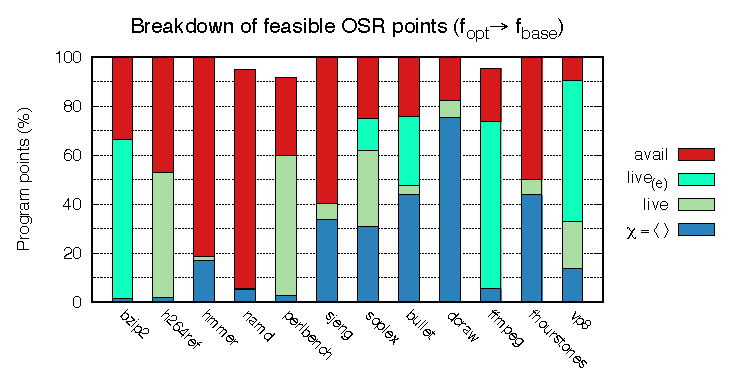
\includegraphics[width=0.8\textwidth]{figures/osr-BC-OtoB/osr-BC-OtoB.eps}
\caption{\protect\label{fig:osr-BC-OtoB} Fraction of program points that are OSR-feasible (from {\em opt} to {\em base}).


}
\end{center}
\end{figure}

\myfigure\ref{fig:osr-BC-OtoB} reports the fraction of OSR points eligible for {\em opt} to {\em base} deoptimization. We observe that the fraction of locations that can fire an OSR with an empty $\chi$ varies significantly from benchmark to benchmark, suggesting a dependence on the structure of the original program.

For $9$ out of $12$ benchmarks, compensation code can be built using only live variables for more than $50\%$ of potential OSR points.
%The assignment step of \reconstruct\ produces on average $2.3$ compensation instructions, with a peak of $5.74$ on \mytt{vp8}.
When the $avail$ version is used, the percentage of feasible OSR points is greater than $90\%$ on all benchmarks and nearly $100\%$ for $9$ out of $12$ of them.

\noindent Results for the $alias$ version of \reconstruct\ are not reported, as they do not improve those for $live_{(e)}$. Indeed, aliasing information is useful when a variable to set at the destination is aliased by multiple variables at the source, which we do not expect to happen in an optimized code.

\begin{table}[!ht]
\begin{center}
\begin{small}
\begin{tabular}{ |c|c|c|c|c|c|c| }
\cline{2-7}
\multicolumn{1}{l|}{} & \multicolumn{2}{c|}{$|\chi|\leftarrow live_{(e)}$} & \multicolumn{2}{c|}{$|\chi|\leftarrow avail$} & \multicolumn{2}{c|}{$|K_{avail}|$} \\
\hline
Benchmark & Avg & Max & Avg & Max & Avg & Max \\
\hline
\hline
bzip2 & 1.55 & 4 & 1.77 & 4 & 1.47 & 4 \\
\hline
h264ref & 4.46 & 9 & 2.82 & 9 & 1.45 & 7 \\
\hline
hmmer & 1 & 1 & 1 & 1 & 1.02 & 2 \\
\hline
namd & 1.5 & 2 & 5.93 & 15 & 4.74 & 18\\
\hline
perlbench & 4.09 & 12 & 4.22 & 12 & 1.37 & 11 \\
\hline
sjeng & 1.29 & 2 & 1.67 & 11 & 4.09 & 14 \\
\hline
soplex & 3.3 & 4 & 3.3 & 4 & 1.00 & 1 \\
\hline
bullet & 1 & 1 & 1.26 & 3 & 1.14 & 2 \\
\hline
dcraw & 1.68 & 2 & 3.84 & 6 & 4.06 & 8 \\
\hline
ffmpeg & 1.94 & 5 & 1.95 & 6 & 1.08 & 4 \\
\hline
fhourstones & 0 & 0 & 1.12 & 4 & 1.42 & 4 \\
\hline
vp8 & 5.74 & 13 & 5.51 & 13 & 1.18 & 5 \\
\hline
\hline
Avg & {\bf 2.30} & 4.58 & {\bf 2.87} & 7.33 & {\bf 2.00} & 6.67 \\
\hline
\end{tabular}
\end{small}
\end{center}
\caption{\label{tab:OSR-alC-prologue-OtoB} Average and peak size $|\chi|$ of the compensation code generated by the $live_{(e)}$ and $avail$ versions of algorithm \reconstruct. $|K_{avail}|$ is the size of the set of variables that we should artificially keep alive in order to make program points represented by white bars in \myfigure\ref{fig:osr-BC-OtoB} feasible for an OSR from {\em opt} to {\em base}.}
\end{table}

\noindent In \mytable\ref{tab:OSR-alC-prologue-OtoB} we report the average and peak size of the compensation code $\chi$ generated by the $live_{(e)}$ and $avail$ variants of \reconstruct\ across feasible OSR points, along with the average and peak number of available variables for which $avail$ artificially extends liveness to support OSR at program points represented by white bars in \myfigure\ref{fig:osr-BC-OtoB}. We observe that, compare to the {\em base}-to-{\em opt} case, the size of the compensation code is much smaller, suggesting that shorter portions of executions need to be reconstructed when ``OSR-ing'' to less optimized code.

Note that the $0$ values reported for \mytt{fhourstones} in the $live_{(e)}$ scenario do not imply that state compensation is not required. In fact, the algorithm detected that each variable $v$ to assign at the OSR landing pad for which no live counterpart was available at the source location, could be initialized with the value of either a (non-live) function argument or some live variable when $v$ is a constant $\phi$-node. In LLVM IR assignments of the form \mytt{x:=y} are not allowed, since all uses of \mytt{x} can simply be replaced with uses of \mytt{y}: for this reason, a \mytt{RAUW(x,y)} operation is performed on the body of the continuation function $f'$, where \mytt{y} is a live value transferred as argument for $f'$, and no instruction is added to the OSR entry block of $f'$.

\subsection{Discussion}
We have seen that common compiler transformations can significantly affect the live state of a program across its locations. The four versions of algorithm \reconstruct\ that we have implemented can generate compensation code automatically by recursively reassembling portions of the state for the target function.

OSR is enabled almost everywhere by the $avail$ version of the algorithm. Figures reported in \mytable\ref{tab:OSR-alC-prologue-BtoO,tab:OSR-alC-prologue-OtoB} suggest that the size of the set of virtual registers to preserve for an OSR from all supported locations is small: a compiler may thus spill available values that are not already located on the stack. When \reconstruct\ can resort only to live variables, it enables OSR at more than a half of the program locations. We observed that the reconstruction would often fail on an available value coming from a memory \load: we thus believe that the algorithm may significantly benefit from a simple alias analysis to identify safely repeatable \load\ instructions.

%For our benchmarks, we enable OSR from both unoptimized to optimized code and viceversa at more than a half of the program locations using only live variables at the source location, and almost anywhere when \reconstruct\ can access previously computed results that are still available.
\fi

\section{Conclusions}
The experimental studies presented in this chapter suggest that the ideas from \mychapter\ref{ch:profiling,ch:continuous} can be efficiently implemented in production systems, yielding promising performance results for popular benchmarks. Our performance profiling techniques incur a low run-time overhead that makes them amenable to be used in an adaptive optimization system. \osrkit\ can insert OSR points in both optimized and unoptimized code with a hardly noticeable overhead. We discuss in \mysection\ref{se:CS-matlab} an example of effective adaptive optimization enabled by it. The \buildcomp\ algorithm for automatic compensation code generations allowed OSR to be performed at a very large fraction of program locations in our experiments. \mysection\ref{se:CS-debug} illustrates a case study on an use of the algorithm to improve optimized code debugging.

\chapter{Case Studies}

\section{Masked Convolution Filters in Image Processing}

\section{Optimizing Higher-Order Functions in MATLAB}
\chapter{Conclusions and Future Work}
\label{ch:conclusions}

We are confident that the ideas presented in this thesis can contribute to the advances in adaptive optimization technology for modern runtimes.

Collecting accurate profiling information with low overhead is a crucial factor for making online complex optimizations practical. In \mychapter\ref{ch:profiling} we have presented two analysis techniques that rely on elegant algorithmic solutions to profile data coming at a high rate from a large universe.

Our inter-procedural profiling technique enables the identification of most frequently encountered calling contexts without having to maintain the whole calling context tree in main memory - which we show can be impractical for real-world applications. We propose a compact data structure, the Hot Calling Context Tree (HCCT), that can be constructed in small space thanks to the adoption of efficient data streaming algorithms. These algorithms provide us with strong theoretical guarantees on the accuracy and the space requirements of the solution, and operate with a constant per-item processing time.

Our intra-procedural profiling technique extends the well-known Ball-Larus algorithm to cyclic-path profiles, in order to yield more optimization opportunities. We show that cyclic paths can be represented as concatenations of acylic Ball-Larus paths, and that a prefix forest can compactly encode them. We then introduce an intermediate data structure, the $k$-slab forest (\ksf), that can be constructed online with a constant per-item processing time and converted to a prefix forest on demand.

The algorithms behind our two profiling techniques have been implemented in mainstream systems and evaluated against prominent benchmarks. Theoretical predictions are thus reinforced by promising experimental results, showing that our techniques can be used in practical scenarios where previous solutions failed.

In \mychapter\ref{ch:continuous} we have then focused our attention on a main player of adaptive optimization cycles, On-Stack Replacement (OSR), which enables runtimes to divert the execution to freshly generated optimized code using profiling information, or to deoptimize to a different version of the code when conditions change, e.g., when program behavior starts to diverge from the profile significantly.

OSR is not only a great engineering problem, but also an intellectually challenging endeavor. We thus tackle the problem from both a practical and theoretical perspective. We present a new framework for on-stack replacement that combines some of the best practices observed in literature, such as platform independence and the generation of highly optimized continuation functions, with two novel features: the ability to perform OSR at any program location, and a compensation code abstraction to encode changes to the program state, thus increasing the flexibility the OSR mechanism. Experimental results collected on classic benchmarks for our \osrkit\ embodiment in the LLVM compiler toolchain suggest that encoding OSR at intermediate representation level allows the compiler to generate very efficient machinery with a hardly noticeable impact on performance. As the ideas behind our OSR framework are general, we do not foresee any limitation to its adoption in other runtime environments as well.

In the second part of \mychapter\ref{ch:continuous}, we make a first attempt to prove OSR transitions sound. To capture OSR in its full generality, we define a notion of multi-program, and let an oracle decide at each program step in which version of the multi-program execution should continue. We distill the essence of OSR to a simple imperative calculus with an operational semantics. Using program bisimulation, we prove that an OSR can correctly divert execution across program versions if they have been generated using live-variable equivalent transformations. We also present an algorithm that can relieve code optimizers from the burden of generating all the required glue machinery to realign the state during an OSR transition.

There is a trade-off between the number of points where OSR can be correctly fired and the price to pay in terms of space and time in order to support them. Our work lies at the performance-preserving end of the spectrum, supporting OSR transitions in constant time and space: we do not restrict optimizations, and do not require any state logging. To assess the practical impact of this design choice, we analyze experimentally the fraction of program locations where OSR can be efficiently fired in prominent benchmarks across several LLVM optimization passes. Our experiments suggest that bidirectional OSR transitions between rather different program versions can be supported almost everywhere in the code under several classic optimizations.

Finally, we present a number of case studies to investigate the end-to-end utility of the techniques described in this thesis. All of our code is publicly available and, for \kblpp\ and \osrkit, has been endorsed along with the associated experiments in the Artifact Evaluation process of known conferences on programming languages.

\section*{Future Work}
The methodologies and ideas presented in this thesis leave a number of interesting open questions that we hope to address in future work.

We believe that a careful use of data mining techniques has the potential benefit of enabling some previously impossible dynamic program analysis tasks, which would otherwise be too costly. In particular, our techniques could be applied to certain forms of path profiling: e.g., they could help leverage the scalability problems encountered when collecting performance metrics about interprocedural paths (i.e., acyclic paths that may cross procedure boundaries)~\cite{Melski99}. Also, it would be interesting to investigate whether streaming algorithms for weighted item sets might be useful to solve space issues arising in other performance profiling methodologies.

An interesting open question for our multi-iteration path profiling technique is how to use sophisticated sampling techniques (e.g., ~\cite{Arnold01,Zhuang06}) to further reduce the profiling overhead. We have seen that bursting is effective in a context-sensitive profiling scenario. To capture even longer paths, our technique might be extended with pruning heuristics that trade accuracy for a smaller memory footprint in the \ksf\ construction. We also remark that our approach, by decoupling path tracing from profiling, is amenable to multi-core implementations by letting the profiled code and the analysis algorithm run on separate cores using shared buffers. A promising line of research is to explore how to partition the data structures so that portions of the stream buffer can be processed in parallel.

We have seen that our approach to OSR mapping generation relies on the live-variable bisimilarity property for program versions. What are the limitations of our formalism in terms of existing compiler optimizations? What is involved in rethinking existing compiler optimizations in terms of the presented model? Transformations that deeply change the structure of a program, such as aggressive loop optimizations, are not supported at the moment. Indeed, such transformations typically require entire portions of state to be logged in order to support deoptimization, such as in the loop tiling case~\cite{Bhandari15}. Our work is just a scratch off the surface of the fascinating problem of how to dynamically morph one program into another. A deep understanding of the trade-offs between flexibility and time/space requirements of OSR remains a compelling goal for future work.

As a next step on the implementation side, we plan to extend \osrkit\ to generate continuation functions that can be shared by multiple deoptimization points. By adding a dispatcher in the entry block that examines the current OSR source location in order to properly compensate the state and jump to the associated landing pad, a single continuation function might serve more than a deoptimization point. Indeed, when transferring execution to less optimized code we should not worry about a possibly reduced peak performance for the modified continuation function: execution won't likely stay in it for long. Also, in the presence of frequent OSR transitions between pairs of versions, this solution would be very effective when deoptimization does not always occur at the same locations.

%We are aware that \osrkit\ is currently being used in a joint academic-industrial research project for the optimization of the runtime for the R language, and we hope to look at other tools that may use it in the future.

We are aware that \osrkit\ is currently being used in a joint academic-industrial research project for the optimization of the runtime for the R language~\cite{vitek16}, and we hope to look at other tools that may use it in the future.

\backmatter

\bibliographystyle{abbrvnat}
\bibliography{bibliography/biblio.bib}

\end{document}